
\documentclass[11pt,letterpaper]{article}

% =========================================================
% PAQUETES
% =========================================================

\usepackage[utf8]{inputenc}
\usepackage[T1]{fontenc}
\usepackage[spanish]{babel}
\usepackage{geometry}
\usepackage{graphicx}
\usepackage{amsmath}
\usepackage{amssymb}
\usepackage{float}
\usepackage{booktabs}
\usepackage{listings}
\usepackage{xcolor}
\usepackage[hidelinks]{hyperref}

\geometry{margin=2.1cm}

% =========================================================
% CONFIGURACION DEL CODIGO PYTHON
% =========================================================

\lstset{
    language=Python,
    basicstyle=\ttfamily\footnotesize,
    keywordstyle=\color{blue},
    commentstyle=\color{gray},
    stringstyle=\color{red!60!black},
    numbers=left,
    numberstyle=\tiny,
    frame=single,
    breaklines=true,
    showstringspaces=false,
    columns=fullflexible,
    keepspaces=true,
    tabsize=4
}

% =========================================================
% DATOS
% =========================================================

\title{
    Taller 8: Segmentación de Imágenes\\
    \large Detección de puntos, líneas y bordes
}

\author{
    Camilo Eduardo Muñoz Albornoz\\
    Procesamiento Digital de Imágenes\\
    Universidad Tecnológica de Pereira
}

\date{}

\begin{document}

\maketitle

\begin{center}
\textbf{Repositorio del código fuente}\\[0.15cm]

\textbf{Carpeta del Taller 8: }
\href
{https://github.com/CamiloMunozAL/ProcDImagenes/tree/main/taller8}
{\textcolor{blue}{
\underline{\texttt{Carpeta del Taller 8 en GitHub}}
}}

\vspace{0.15cm}

\textbf{Cuaderno Python: }
\href
{https://github.com/CamiloMunozAL/ProcDImagenes/blob/main/taller8/taller8.ipynb}
{\textcolor{blue}{
\underline{\texttt{taller8.ipynb}}
}}
\end{center}

% =========================================================
\begin{abstract}

En este taller se implementaron diferentes algoritmos
de segmentación y detección de características en
imágenes digitales, utilizando principalmente máscaras
espaciales y ciclos en Python.

Se desarrollaron siete ejercicios: detección de puntos
aislados, detección de líneas orientadas y detección
de bordes mediante los operadores Prewitt, Sobel,
Laplaciano, Marr-Hildreth y Canny.

Los algoritmos se probaron con imágenes sintéticas
de puntos, líneas y un cuadrado, además de fotografías
de un campo de estrellas y un paisaje natural.

Los resultados permitieron comprender cómo las
variaciones de intensidad pueden utilizarse para
localizar estructuras en una imagen y cómo el
suavizado, los umbrales y las propiedades de cada
algoritmo influyen en las detecciones obtenidas.

\end{abstract}

% =========================================================
\section{Objetivos}

Los objetivos del taller fueron:

\begin{enumerate}

    \item Implementar mediante ciclos un detector
    de puntos aislados y analizar el efecto de
    eliminar el factor $1/9$ de la máscara.

    \item Implementar un detector de líneas
    horizontales, verticales y diagonales
    mediante máscaras espaciales.

    \item Implementar el operador Prewitt
    para detectar bordes mediante gradientes.

    \item Implementar el operador Sobel
    y analizar su comportamiento en imágenes.

    \item Implementar el operador Laplaciano
    utilizando derivadas de segundo orden.

    \item Implementar una versión del algoritmo
    Marr-Hildreth mediante suavizado Gaussiano,
    Laplaciano y cruces por cero.

    \item Implementar una versión manual del
    detector Canny con $\sigma=5$, incluyendo
    gradiente, supresión de no máximos
    y doble umbral con histéresis.

\end{enumerate}

% =========================================================
\section{Fundamentos teóricos}

\subsection{Segmentación de imágenes}

La segmentación consiste en dividir una imagen
en regiones o identificar estructuras mediante
características como intensidad, color,
textura o cambios entre píxeles.

Existen dos enfoques generales:

\begin{itemize}

    \item \textbf{Similitud:} agrupar píxeles
    con características parecidas.

    \item \textbf{Discontinuidad:} identificar
    cambios importantes que puedan representar
    bordes, líneas o puntos aislados.

\end{itemize}

En este taller se trabajó principalmente
con técnicas basadas en discontinuidades.

Es importante distinguir una región de
un borde: una región contiene un conjunto
de píxeles, mientras que un borde representa
una transición entre zonas.

\subsection{Máscaras espaciales}

Una máscara espacial es una matriz pequeña
de coeficientes que se aplica sobre la
vecindad de cada píxel.

Para una máscara de $3\times3$, la respuesta
en una posición puede calcularse como:

\begin{equation}
R(x,y)=
\sum_{i=-1}^{1}
\sum_{j=-1}^{1}
w(i,j)f(x+i,y+j)
\end{equation}

Donde $f$ representa la imagen y $w$
los coeficientes de la máscara.

Según la organización de estos coeficientes,
podemos detectar puntos aislados,
líneas orientadas o cambios de intensidad.

\subsection{Umbral de detección}

Los filtros generan respuestas numéricas,
pero no todas representan características
que deseamos conservar.

Por eso se utiliza un umbral $T$.

En una detección basada en magnitud:

\begin{equation}
B(x,y)=
\begin{cases}
255, & |R(x,y)|>T\\
0, & |R(x,y)|\leq T
\end{cases}
\end{equation}

Un umbral bajo permite conservar más respuestas,
incluyendo posibles variaciones pequeñas o ruido.

Un umbral alto reduce la cantidad de detecciones,
pero también puede eliminar características
relevantes.

\subsection{Derivadas y gradientes}

Los bordes suelen aparecer donde existe
una variación importante de intensidad.

Los operadores de primer orden,
como Prewitt y Sobel, aproximan
las derivadas en dos direcciones:

\[
G_x=\frac{\partial f}{\partial x},
\qquad
G_y=\frac{\partial f}{\partial y}
\]

La magnitud del gradiente se calcula mediante:

\begin{equation}
G(x,y)=\sqrt{G_x^2+G_y^2}
\end{equation}

La orientación se obtiene con:

\begin{equation}
\theta(x,y)=
\operatorname{atan2}(G_y,G_x)
\end{equation}

La magnitud indica la intensidad del cambio
y la orientación señala la dirección
en que la intensidad aumenta más rápidamente.

Por otro lado, el operador Laplaciano
utiliza derivadas de segundo orden:

\begin{equation}
\nabla^2f=
\frac{\partial^2 f}{\partial x^2}
+
\frac{\partial^2 f}{\partial y^2}
\end{equation}

Estas derivadas pueden responder con fuerza
a variaciones pequeñas de intensidad,
por lo que suelen combinarse con suavizado
cuando la imagen presenta mucho detalle.

\subsection{Suavizado y detección de bordes}

El filtro Gaussiano reduce pequeñas
variaciones de intensidad antes de aplicar
un detector de bordes.

Su expresión es:

\begin{equation}
G_\sigma(x,y)=
\frac{1}{2\pi\sigma^2}
e^{-\frac{x^2+y^2}{2\sigma^2}}
\end{equation}

El parámetro $\sigma$ controla
la extensión del suavizado.

Un valor mayor produce una reducción
más intensa de detalles pequeños,
aunque también puede eliminar bordes finos.

Los algoritmos Marr-Hildreth y Canny
utilizan suavizado como parte
de sus procedimientos de detección.

% =========================================================
\section{Imágenes y metodología}

\subsection{Imágenes utilizadas}

Se seleccionaron imágenes sintéticas
y fotografías reales para comprobar
los algoritmos en diferentes condiciones.

\begin{itemize}

    \item \textbf{Puntos aislados:}
    imagen sintética de $32\times32$
    píxeles con dos puntos brillantes
    y un punto oscuro sobre fondo gris.

    \item \textbf{Campo de estrellas:}
    fotografía en escala de grises
    utilizada para evaluar la detección
    de pequeñas variaciones de intensidad.

    \item \textbf{Líneas orientadas:}
    imagen sintética de $256\times256$
    píxeles con cuatro líneas blancas:
    horizontal, vertical y dos diagonales.

    \item \textbf{Cuadrado:}
    imagen sintética de $256\times256$
    píxeles con un cuadrado blanco
    sobre fondo negro.

    \item \textbf{Paisaje natural:}
    fotografía en escala de grises
    que contiene montañas, árboles,
    vegetación y un lago con reflejos.

\end{itemize}

Las imágenes sintéticas se crearon mediante
NumPy. Las fotografías se cargaron en escala
de grises utilizando OpenCV.

Los resultados se visualizaron con Matplotlib
y se guardaron como figuras para incluirlas
en este informe.

\subsection{Preparación de las imágenes}

\begin{lstlisting}
import numpy as np
import cv2

# Imagen con puntos aislados
imagen_prueba = np.full(
    (32, 32), 50, dtype=np.uint8
)

imagen_prueba[8, 8] = 255
imagen_prueba[16, 24] = 230
imagen_prueba[24, 12] = 0

# Campo de estrellas
imagen_estrellas = cv2.imread(
    "images/CampoEstrellas.png",
    cv2.IMREAD_GRAYSCALE
)

# Imagen con cuatro lineas
imagen_lineas = np.zeros(
    (256, 256), dtype=np.uint8
)

imagen_lineas[40, 20:100] = 255
imagen_lineas[20:100, 180] = 255

for i in range(65):
    imagen_lineas[125+i, 20+i] = 255
    imagen_lineas[190-i, 160+i] = 255

# Cuadrado
cuadrado = np.zeros(
    (256, 256), dtype=np.uint8
)

cuadrado[64:192, 64:192] = 255

# Paisaje
paisaje = cv2.imread(
    "images/paisaje.png",
    cv2.IMREAD_GRAYSCALE
)

if imagen_estrellas is None or paisaje is None:
    raise FileNotFoundError(
        "No se encontraron las fotografias"
    )
\end{lstlisting}

Los algoritmos se desarrollaron mediante
ciclos para recorrer los píxeles y aplicar
las máscaras correspondientes.

En las funciones se utilizaron matrices
de tipo \texttt{float64} para almacenar
respuestas que pueden ser negativas
o superiores a 255.

% =========================================================
\section{Desarrollo y resultados}

% ---------------------------------------------------------
\subsection{Punto 1: Detección de puntos aislados}

\subsubsection*{Objetivo}

Desarrollar una función basada en ciclos
para detectar puntos aislados y comparar
su funcionamiento con y sin el factor $1/9$.

\subsubsection*{Fundamento}

Se utilizó la máscara:

\begin{equation}
W=
\begin{bmatrix}
-1&-1&-1\\
-1&8&-1\\
-1&-1&-1
\end{bmatrix}
\end{equation}

Esta compara la intensidad del píxel central
con la suma de sus ocho vecinos.

Una respuesta positiva elevada puede
corresponder a un punto brillante,
mientras que una respuesta negativa
elevada en magnitud puede corresponder
a un punto oscuro.

La versión con factor $1/9$ se obtiene
dividiendo la máscara entre nueve.

\subsubsection*{Implementación}

\begin{lstlisting}
def detectar_puntos_aislados(
    imagen, umbral, usar_promedio=True
):

    if imagen is None:
        raise ValueError(
            "La imagen no se cargo"
        )

    if umbral < 0:
        raise ValueError(
            "El umbral debe ser positivo"
        )

    filas, columnas = imagen.shape

    respuestas = np.zeros(
        (filas, columnas),
        dtype=np.float64
    )

    puntos_detectados = np.zeros(
        (filas, columnas),
        dtype=np.uint8
    )

    mascara = np.array([
        [-1, -1, -1],
        [-1,  8, -1],
        [-1, -1, -1]
    ], dtype=np.float64)

    if usar_promedio:
        mascara = mascara / 9.0

    for fila in range(1, filas - 1):
        for columna in range(1, columnas - 1):

            suma = 0.0

            for i in range(-1, 2):
                for j in range(-1, 2):

                    pixel = float(
                        imagen[fila+i, columna+j]
                    )

                    peso = mascara[i+1, j+1]

                    suma += pixel * peso

            respuestas[fila, columna] = suma

            if abs(suma) > umbral:
                puntos_detectados[
                    fila, columna
                ] = 255

    return respuestas, puntos_detectados
\end{lstlisting}

\subsubsection*{Resultados y análisis}

\begin{figure}[H]
    \centering
    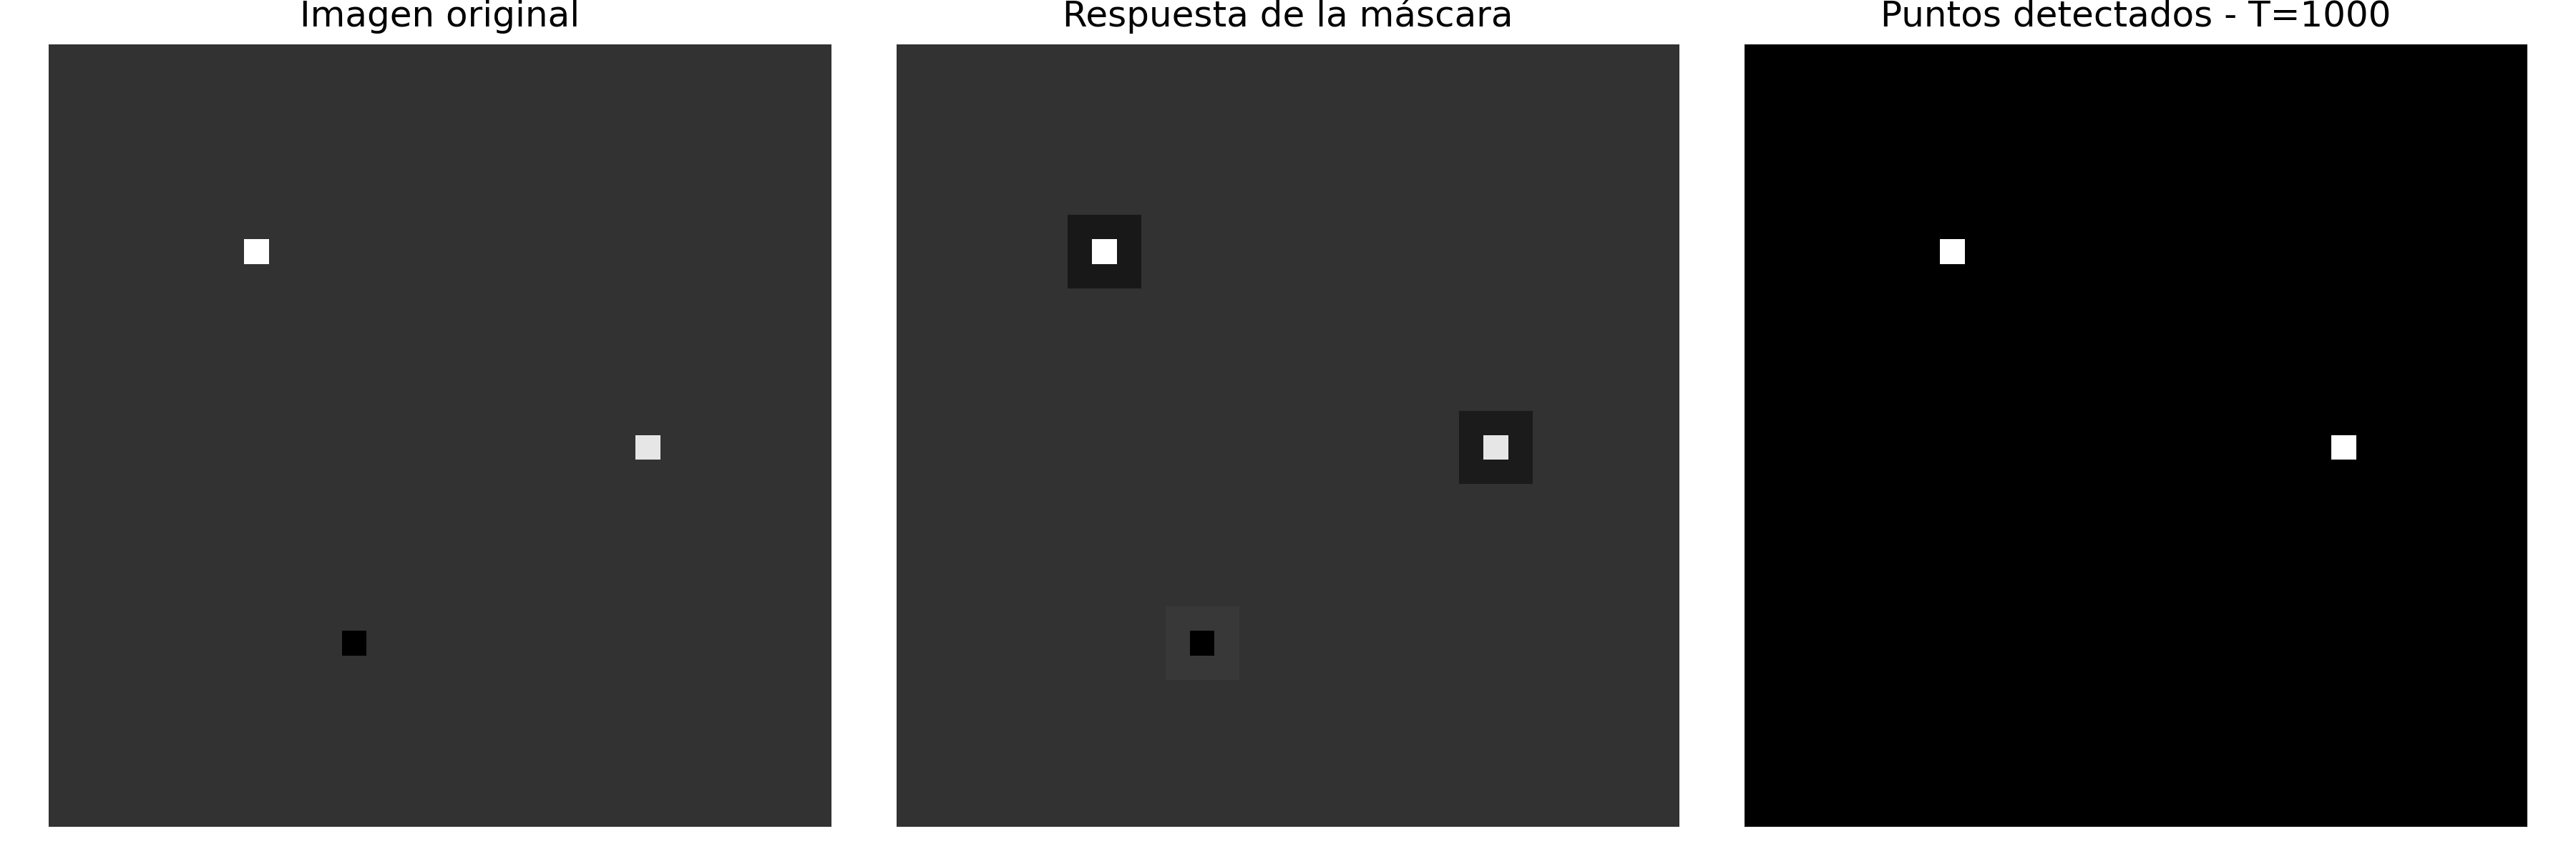
\includegraphics[width=0.95\textwidth]
    {../results/deteccion_puntos_aislados.png}
    \caption{Prueba de detección de puntos
    en una imagen sintética de $32\times32$.}
    \label{fig:puntos_sinteticos}
\end{figure}

En la imagen sintética se detectaron
los dos puntos brillantes utilizando
un umbral de 1000 sin el factor $1/9$.

El punto oscuro no superó dicho umbral.

Las respuestas centrales fueron:

\begin{table}[H]
\centering
\caption{Respuestas en los puntos de prueba.}
\begin{tabular}{lcc}
\toprule
\textbf{Punto} &
\textbf{Intensidad} &
\textbf{Respuesta}\\
\midrule
Brillante 1 & 255 & 1640\\
Brillante 2 & 230 & 1440\\
Oscuro & 0 & -400\\
\bottomrule
\end{tabular}
\end{table}

También se observaron respuestas de
signo contrario en los píxeles vecinos,
debido a los coeficientes negativos
de la máscara.

Posteriormente, se aplicó el detector
a un campo de estrellas.

\begin{figure}[H]
    \centering
    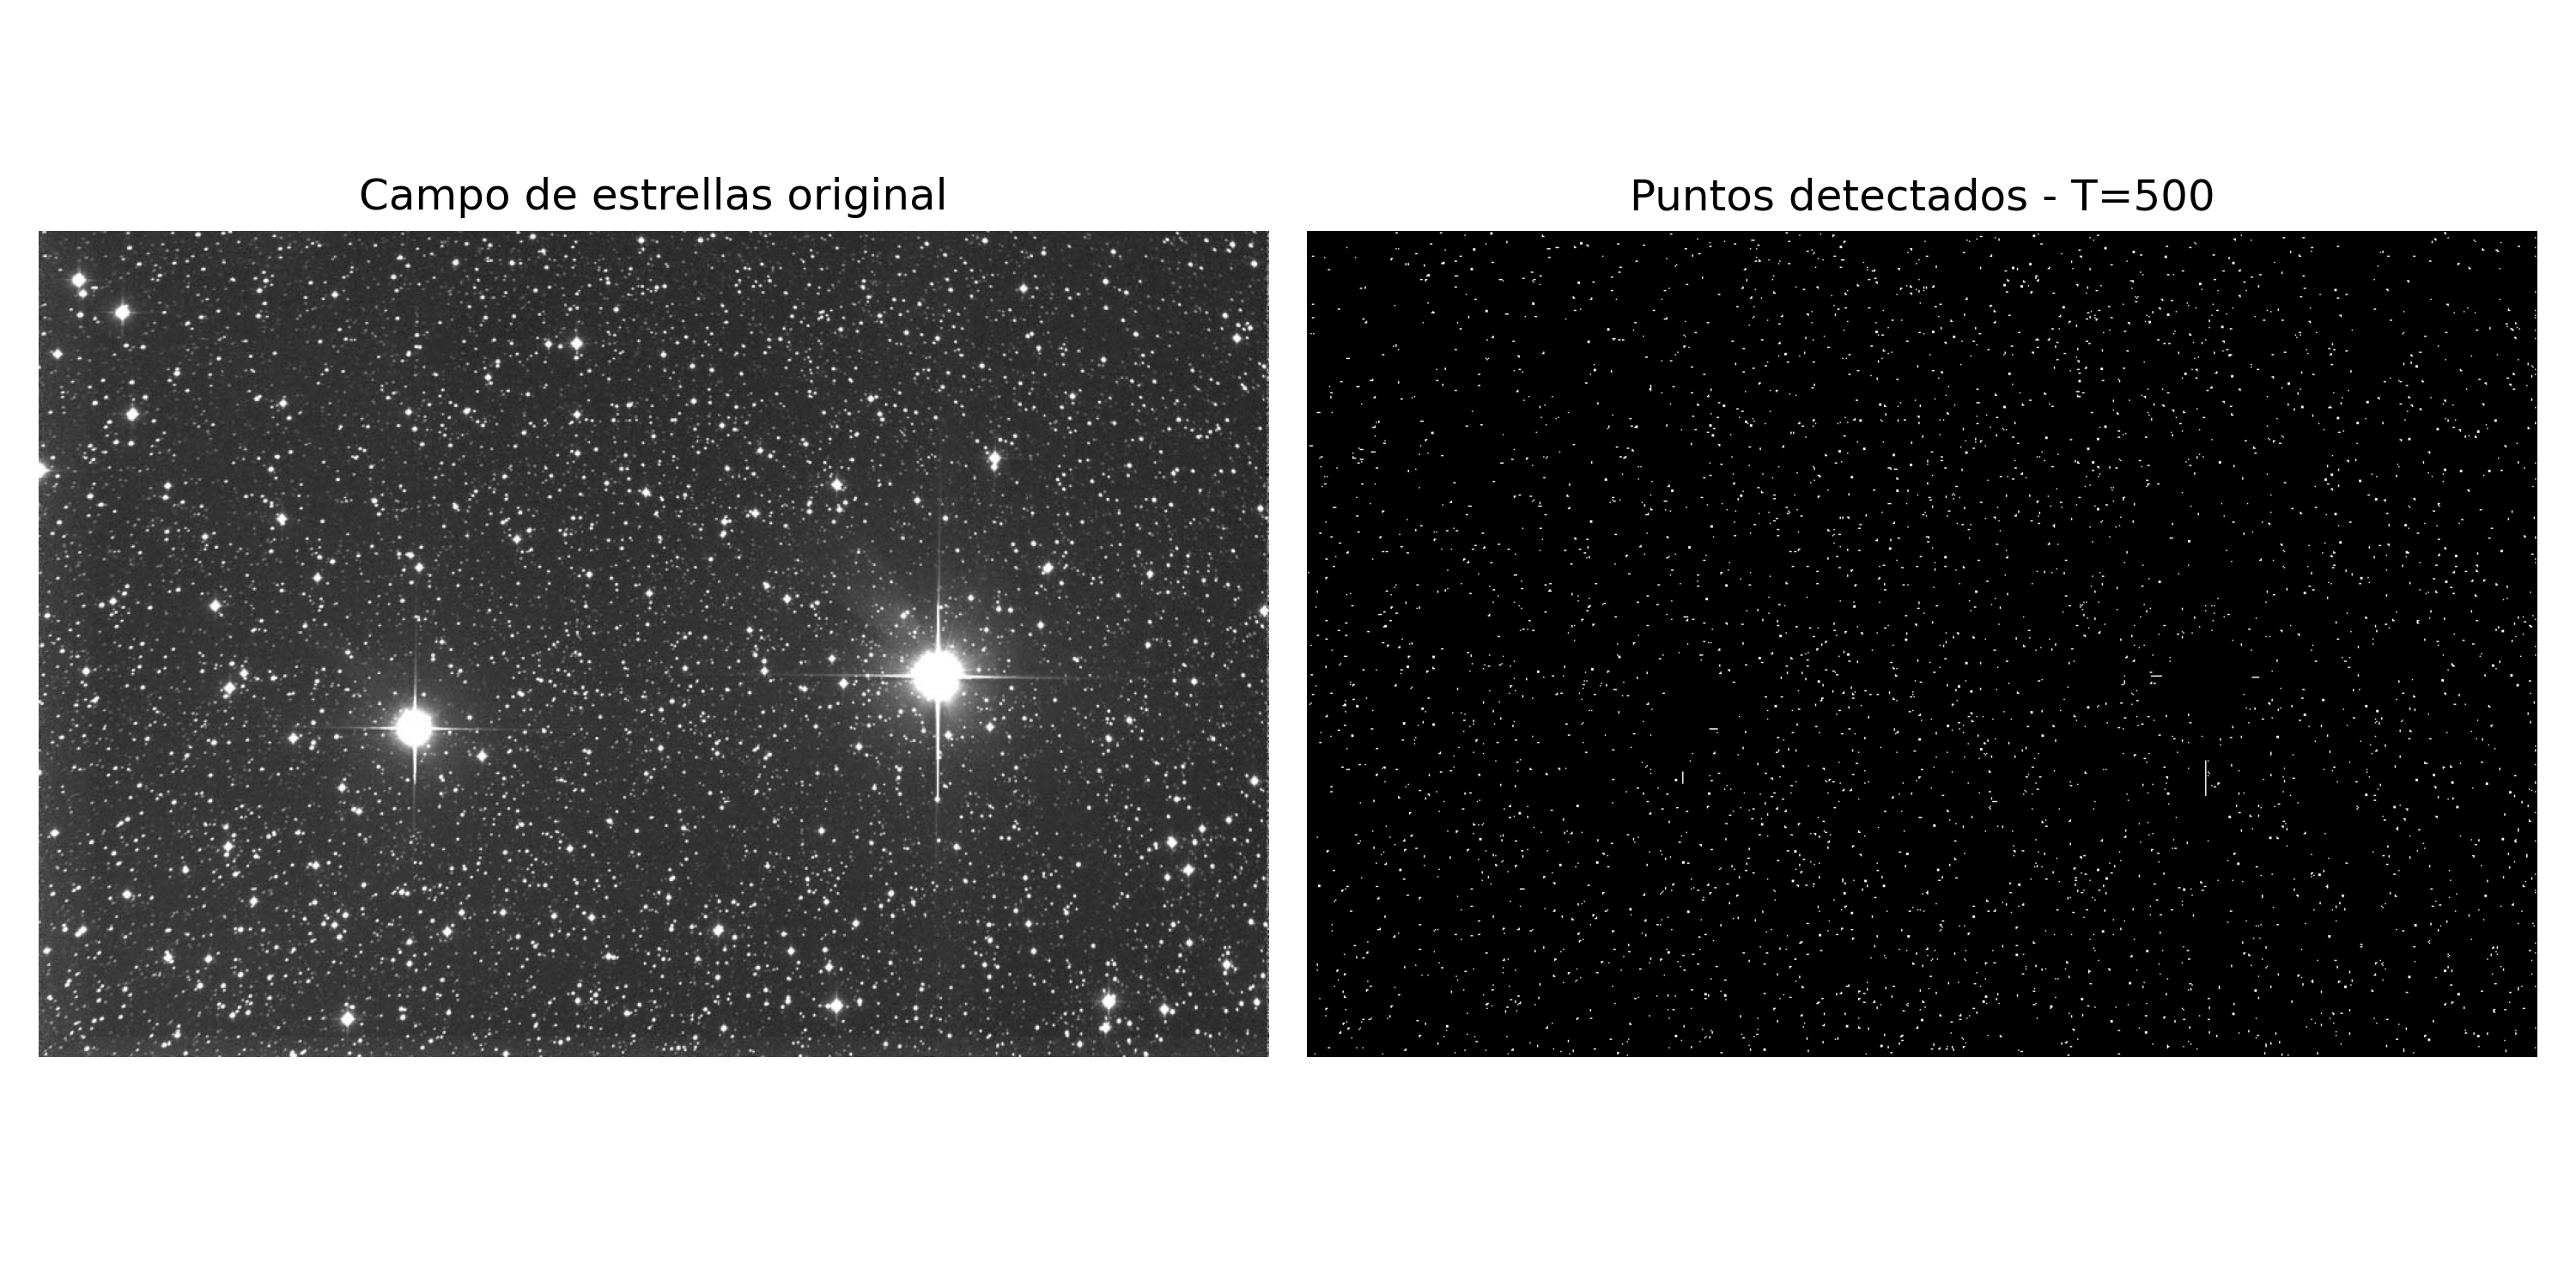
\includegraphics[width=0.95\textwidth]
    {../results/deteccion_puntos_estrellas.png}
    \caption{Detección de puntos en
    una fotografía de un campo de estrellas.}
    \label{fig:puntos_estrellas}
\end{figure}

Para cumplir la comparación del ejercicio,
se ejecutó el algoritmo con y sin
el factor $1/9$, manteniendo el mismo
umbral de 500.

\begin{figure}[H]
    \centering
    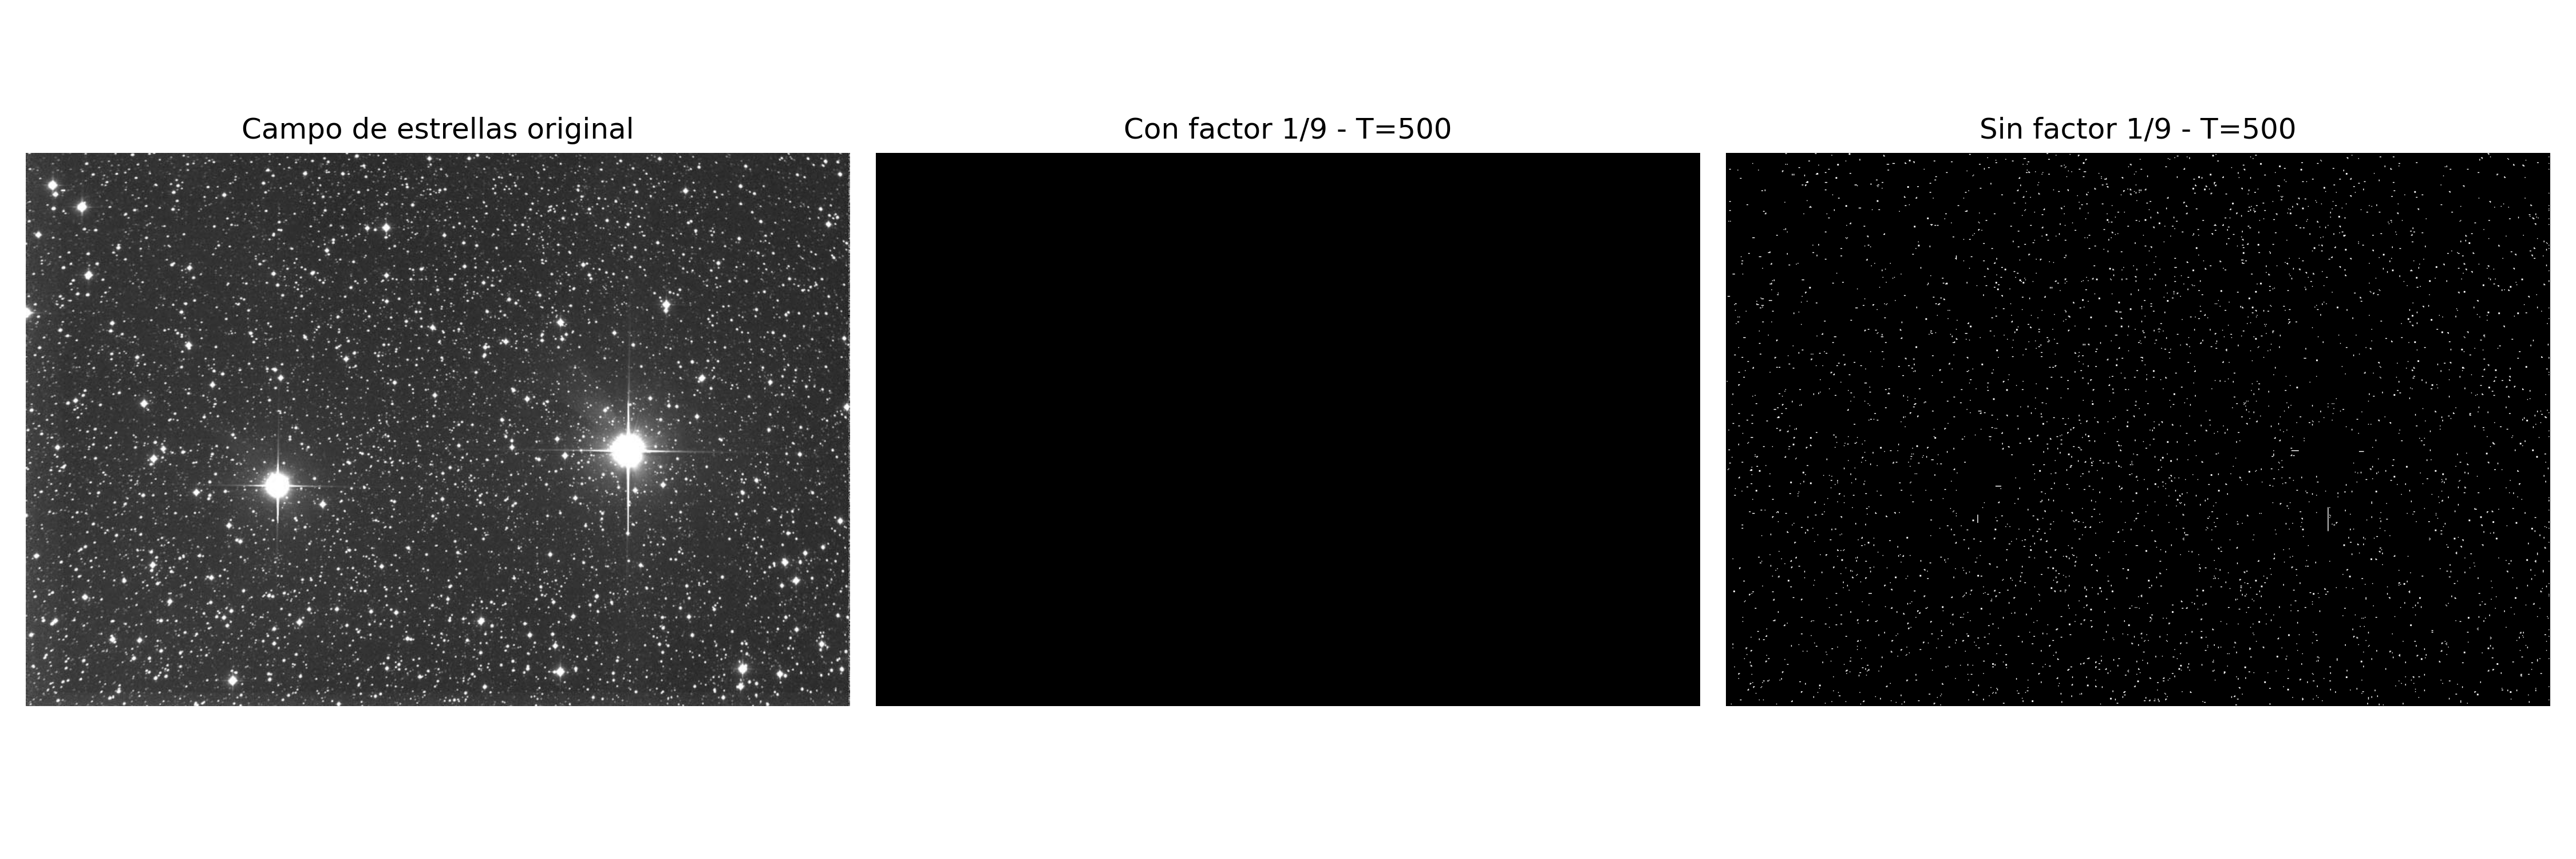
\includegraphics[width=\textwidth]
    {../results/deteccion_estrellas_comparacion.png}
    \caption{Comparación de detecciones
    con y sin el factor $1/9$.}
    \label{fig:puntos_factor}
\end{figure}

Los resultados fueron:

\begin{table}[H]
\centering
\caption{Detecciones con umbral 500.}
\begin{tabular}{lc}
\toprule
\textbf{Configuración} &
\textbf{Píxeles detectados}\\
\midrule
Con factor $1/9$ & 0\\
Sin factor $1/9$ & 6797\\
\bottomrule
\end{tabular}
\end{table}

Eliminar el factor multiplica las respuestas
numéricas por nueve.

Por tanto, si se mantiene el mismo umbral,
más posiciones pueden superar el criterio
de detección.

Esto no implica que se hayan identificado
6797 estrellas: el número corresponde
a píxeles que superaron el umbral,
incluyendo posibles respuestas al ruido
y a otras variaciones de intensidad.

\textbf{Conclusión del punto:}
la máscara permite detectar variaciones
locales importantes. El factor $1/9$
cambia la escala de la respuesta,
mientras que el umbral determina
cuáles posiciones se marcan.

% ---------------------------------------------------------
\subsection{Punto 2: Detección de líneas}

\subsubsection*{Objetivo}

Desarrollar una función basada en ciclos
para identificar líneas horizontales,
verticales y diagonales mediante
máscaras espaciales.

\subsubsection*{Fundamento}

Las máscaras asignan coeficientes positivos
a los píxeles que deberían formar una línea
y coeficientes negativos a su entorno.

Se utilizaron las siguientes máscaras:

\[
W_h=
\begin{bmatrix}
-1&-1&-1\\
2&2&2\\
-1&-1&-1
\end{bmatrix}
\qquad
W_v=
\begin{bmatrix}
-1&2&-1\\
-1&2&-1\\
-1&2&-1
\end{bmatrix}
\]

\[
W_{\backslash}=
\begin{bmatrix}
2&-1&-1\\
-1&2&-1\\
-1&-1&2
\end{bmatrix}
\qquad
W_{/}=
\begin{bmatrix}
-1&-1&2\\
-1&2&-1\\
2&-1&-1
\end{bmatrix}
\]

\subsubsection*{Implementación}

\begin{lstlisting}
def detectar_lineas(imagen, mascara, umbral):

    if imagen is None:
        raise ValueError(
            "La imagen no se cargo"
        )

    filas, columnas = imagen.shape

    respuestas = np.zeros(
        (filas, columnas),
        dtype=np.float64
    )

    lineas_detectadas = np.zeros(
        (filas, columnas),
        dtype=np.uint8
    )

    for fila in range(1, filas - 1):
        for columna in range(1, columnas - 1):

            suma = 0.0

            for i in range(-1, 2):
                for j in range(-1, 2):

                    pixel = float(
                        imagen[fila+i, columna+j]
                    )

                    peso = mascara[i+1, j+1]

                    suma += pixel * peso

            respuestas[fila, columna] = suma

            if suma > umbral:
                lineas_detectadas[
                    fila, columna
                ] = 255

    return respuestas, lineas_detectadas
\end{lstlisting}

Las cuatro máscaras se definieron y
aplicaron utilizando un umbral de 700.

\begin{lstlisting}
mascaras_lineas = {
    "Horizontal": np.array([
        [-1, -1, -1],
        [ 2,  2,  2],
        [-1, -1, -1]
    ]),

    "Vertical": np.array([
        [-1,  2, -1],
        [-1,  2, -1],
        [-1,  2, -1]
    ]),

    "Diagonal descendente": np.array([
        [ 2, -1, -1],
        [-1,  2, -1],
        [-1, -1,  2]
    ]),

    "Diagonal ascendente": np.array([
        [-1, -1,  2],
        [-1,  2, -1],
        [ 2, -1, -1]
    ])
}

resultados_lineas = {}

for nombre, mascara in mascaras_lineas.items():

    respuesta, deteccion = detectar_lineas(
        imagen_lineas,
        mascara,
        umbral=700
    )

    resultados_lineas[nombre] = deteccion
\end{lstlisting}

\subsubsection*{Resultados y análisis}

\begin{figure}[H]
    \centering
    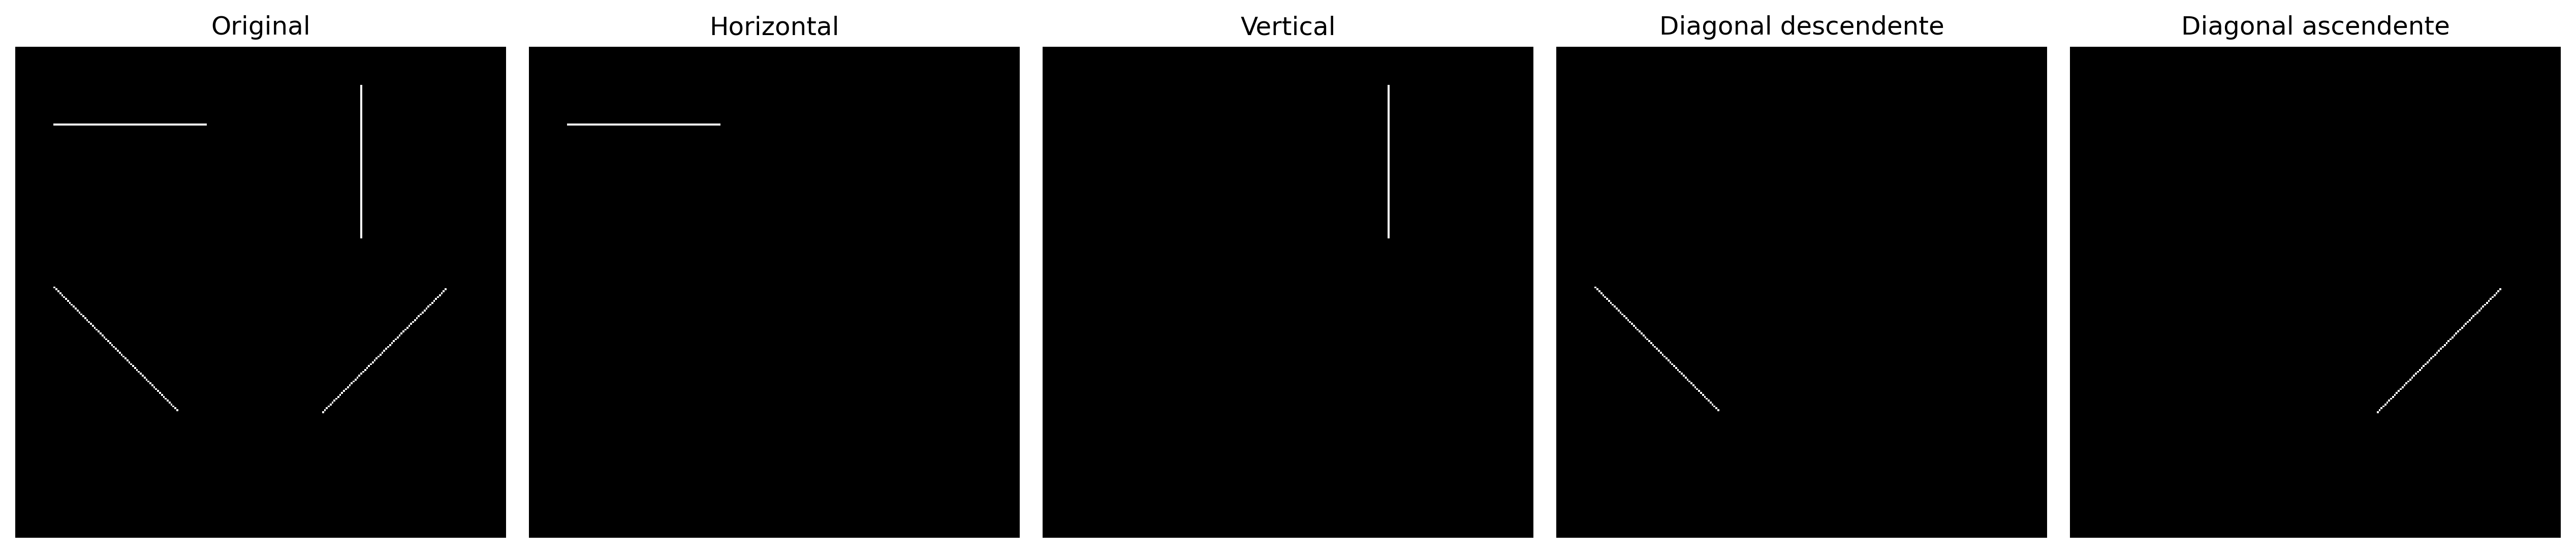
\includegraphics[width=\textwidth]
    {../results/deteccion_lineas.png}
    \caption{Detección de cuatro orientaciones
    en una imagen sintética.}
    \label{fig:lineas}
\end{figure}

Cada máscara identificó correctamente
la línea correspondiente a su orientación.

En el centro de las cuatro líneas se obtuvo
una respuesta de 1530, superior al
umbral de 700.

Este valor aparece porque los tres píxeles
blancos coinciden con los coeficientes
positivos de cada máscara:

\[
R=3(2)(255)=1530
\]

\textbf{Conclusión del punto:}
la organización de los coeficientes de
una máscara determina la orientación
a la que responde.

Los filtros analizan patrones locales,
por lo que en imágenes complejas
también podrían producir respuestas
sobre otras estructuras similares.

% ---------------------------------------------------------
\subsection{Punto 3: Detector Prewitt}

\subsubsection*{Objetivo}

Implementar el operador Prewitt
para detectar bordes mediante
gradientes horizontales y verticales.

\subsubsection*{Fundamento}

Se utilizaron las máscaras:

\[
P_x=
\begin{bmatrix}
-1&0&1\\
-1&0&1\\
-1&0&1
\end{bmatrix}
\qquad
P_y=
\begin{bmatrix}
-1&-1&-1\\
0&0&0\\
1&1&1
\end{bmatrix}
\]

Las respuestas se combinaron
mediante la magnitud del gradiente.

\subsubsection*{Implementación}

\begin{lstlisting}
def detectar_bordes_prewitt(imagen):

    if imagen is None:
        raise ValueError(
            "La imagen no se cargo"
        )

    filas, columnas = imagen.shape

    mascara_x = np.array([
        [-1, 0, 1],
        [-1, 0, 1],
        [-1, 0, 1]
    ])

    mascara_y = np.array([
        [-1, -1, -1],
        [ 0,  0,  0],
        [ 1,  1,  1]
    ])

    gx = np.zeros(
        (filas, columnas),
        dtype=np.float64
    )

    gy = np.zeros(
        (filas, columnas),
        dtype=np.float64
    )

    for fila in range(1, filas - 1):
        for columna in range(1, columnas - 1):

            suma_x = 0.0
            suma_y = 0.0

            for i in range(-1, 2):
                for j in range(-1, 2):

                    pixel = float(
                        imagen[fila+i, columna+j]
                    )

                    suma_x += (
                        pixel * mascara_x[i+1, j+1]
                    )

                    suma_y += (
                        pixel * mascara_y[i+1, j+1]
                    )

            gx[fila, columna] = suma_x
            gy[fila, columna] = suma_y

    magnitud = np.sqrt(gx**2 + gy**2)

    return magnitud, gx, gy
\end{lstlisting}

\subsubsection*{Resultados y análisis}

\begin{figure}[H]
    \centering
    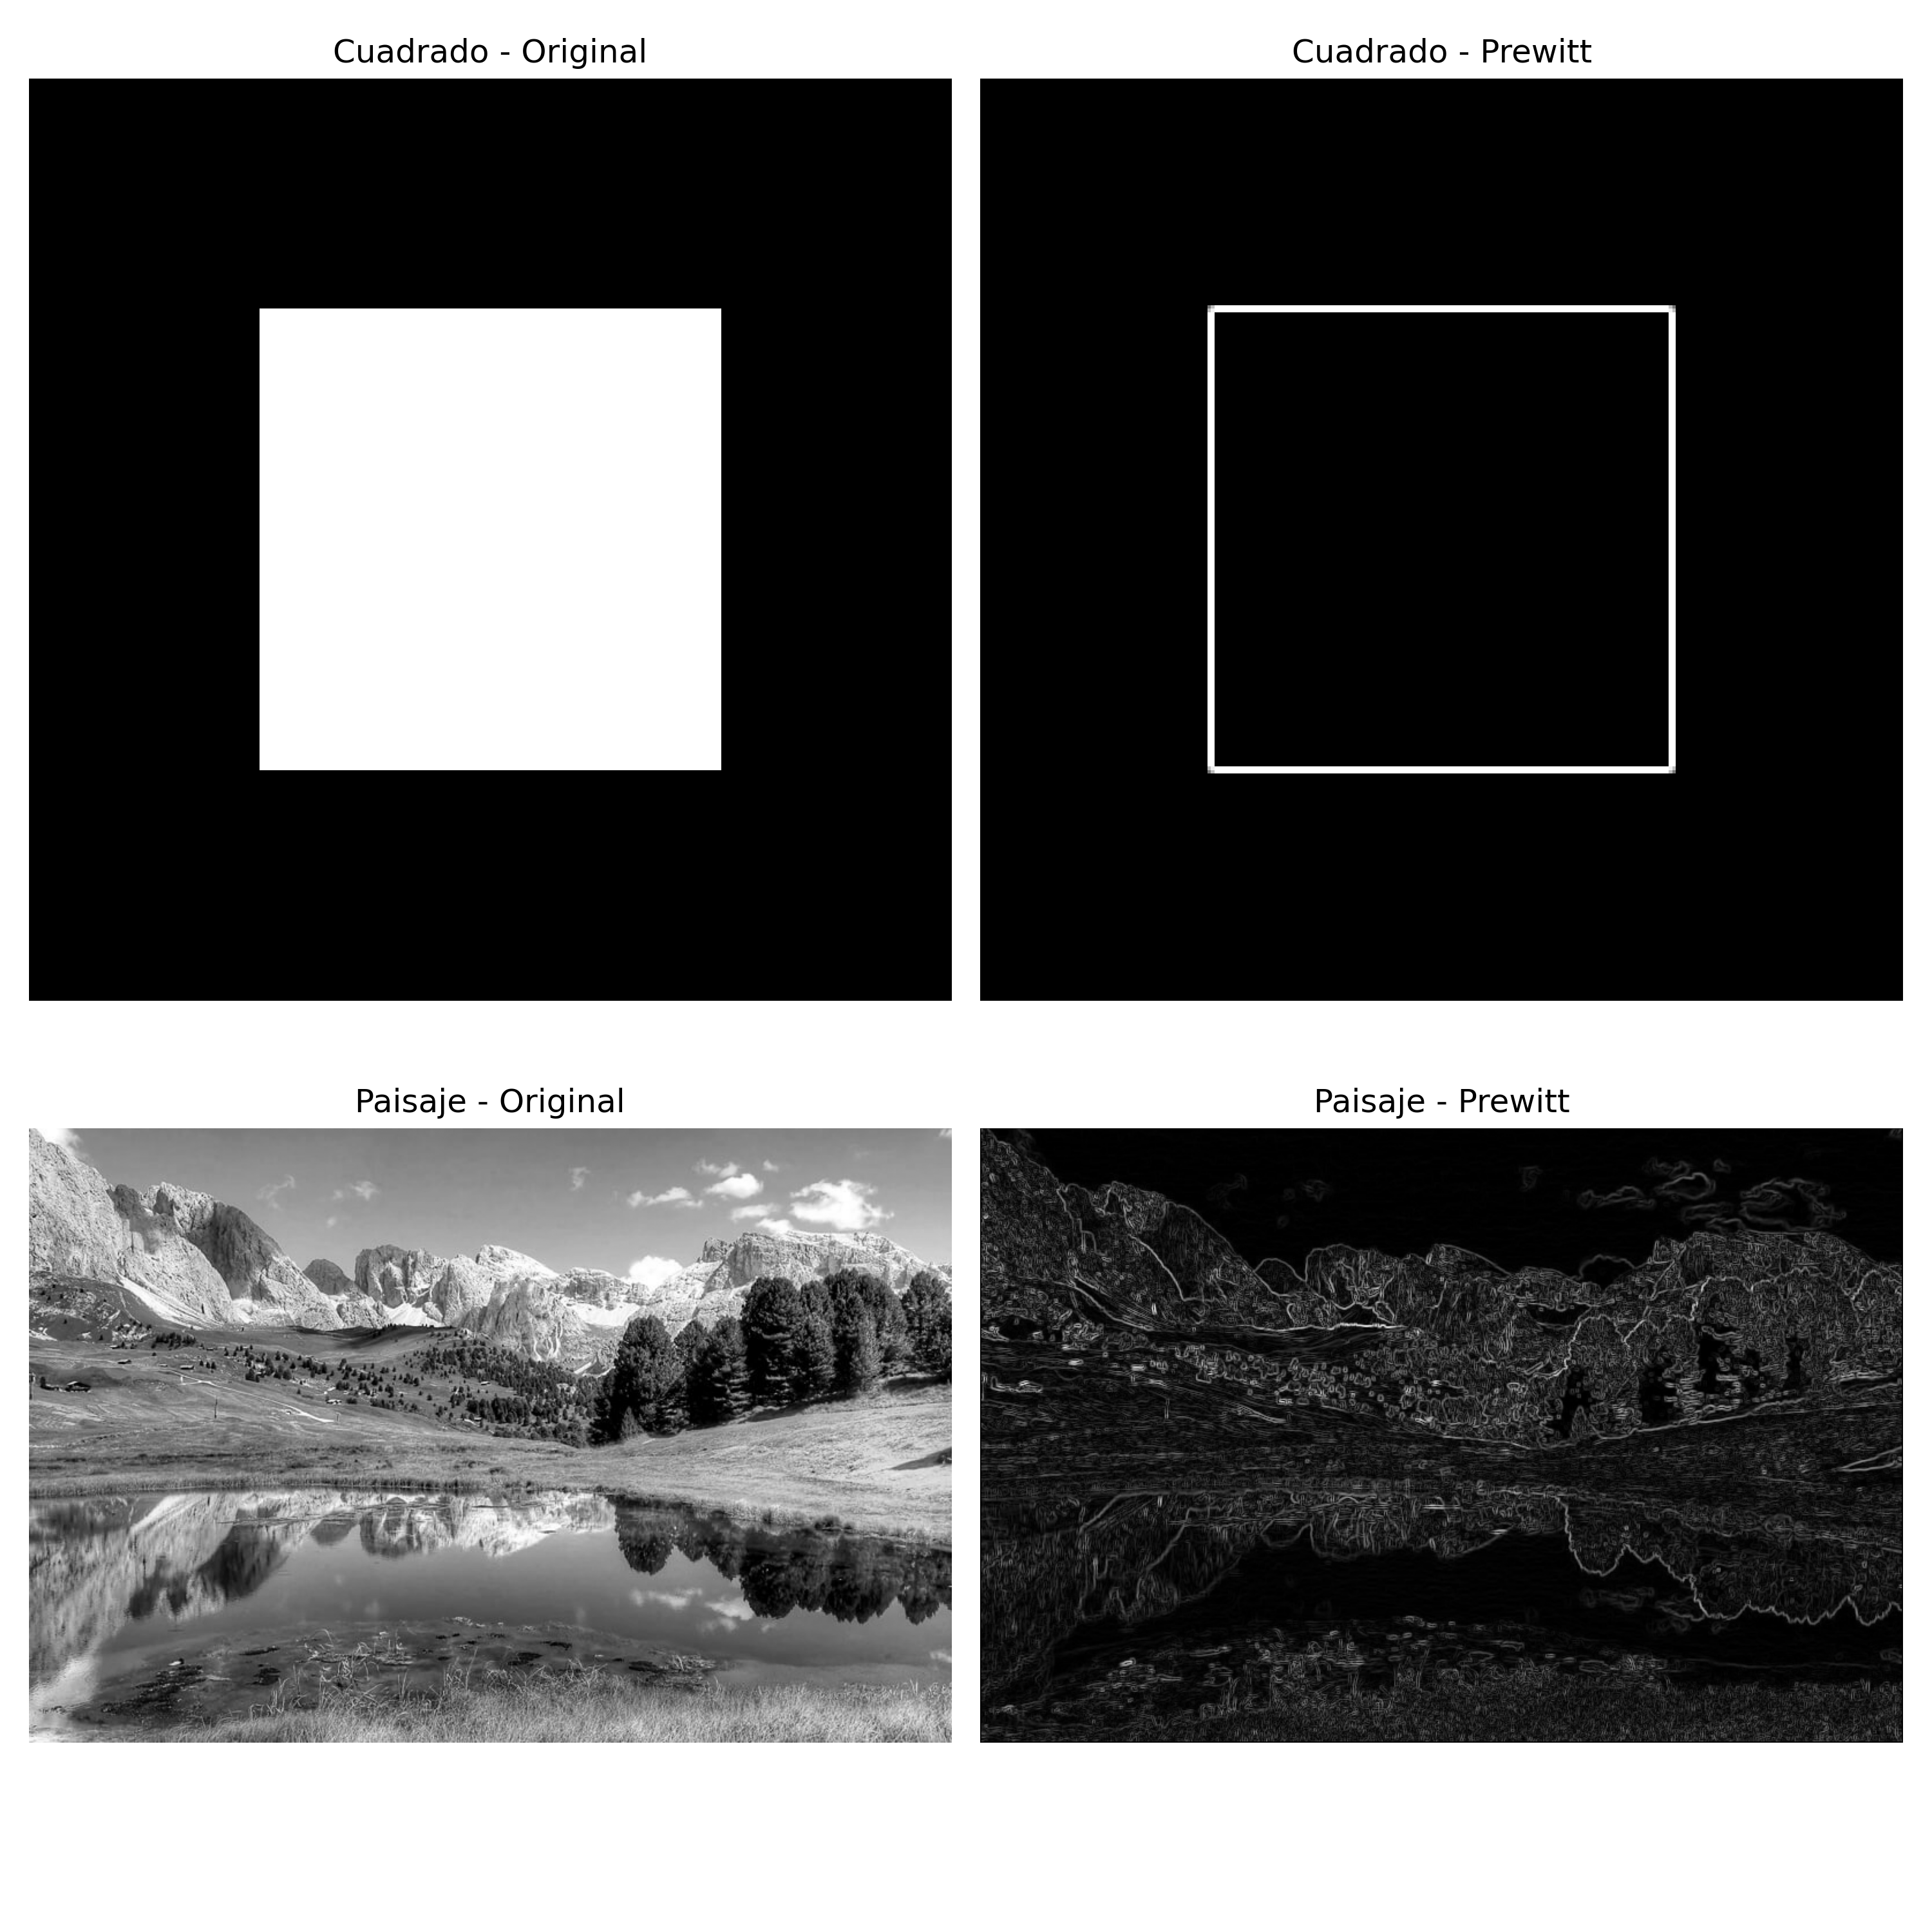
\includegraphics[width=0.90\textwidth]
    {../results/deteccion_bordes_prewitt.png}
    \caption{Detección de bordes con Prewitt
    sobre el cuadrado y el paisaje.}
    \label{fig:prewitt}
\end{figure}

En el cuadrado se identificaron sus
cuatro bordes, mientras que el interior
y el fondo permanecieron oscuros.

En el paisaje se destacaron contornos
de montañas, árboles, vegetación
y reflejos en el agua.

También aparecieron respuestas
relacionadas con texturas pequeñas.

\textbf{Conclusión del punto:}
Prewitt permite identificar transiciones
de intensidad en distintas orientaciones,
pero no distingue automáticamente
entre contornos principales y texturas.

% ---------------------------------------------------------
\subsection{Punto 4: Detector Sobel}

\subsubsection*{Objetivo}

Implementar el operador Sobel mediante
ciclos y evaluar sus resultados
sobre el cuadrado y el paisaje.

\subsubsection*{Fundamento}

Sobel utiliza máscaras similares
a Prewitt, pero asigna mayor peso
a la fila o columna central:

\[
S_x=
\begin{bmatrix}
-1&0&1\\
-2&0&2\\
-1&0&1
\end{bmatrix}
\qquad
S_y=
\begin{bmatrix}
-1&-2&-1\\
0&0&0\\
1&2&1
\end{bmatrix}
\]

\subsubsection*{Implementación}

\begin{lstlisting}
def detectar_bordes_sobel(imagen):

    if imagen is None:
        raise ValueError(
            "La imagen no se cargo"
        )

    filas, columnas = imagen.shape

    mascara_x = np.array([
        [-1, 0, 1],
        [-2, 0, 2],
        [-1, 0, 1]
    ])

    mascara_y = np.array([
        [-1, -2, -1],
        [ 0,  0,  0],
        [ 1,  2,  1]
    ])

    gx = np.zeros(
        (filas, columnas),
        dtype=np.float64
    )

    gy = np.zeros(
        (filas, columnas),
        dtype=np.float64
    )

    for fila in range(1, filas - 1):
        for columna in range(1, columnas - 1):

            suma_x = 0.0
            suma_y = 0.0

            for i in range(-1, 2):
                for j in range(-1, 2):

                    pixel = float(
                        imagen[fila+i, columna+j]
                    )

                    suma_x += (
                        pixel * mascara_x[i+1, j+1]
                    )

                    suma_y += (
                        pixel * mascara_y[i+1, j+1]
                    )

            gx[fila, columna] = suma_x
            gy[fila, columna] = suma_y

    magnitud = np.sqrt(gx**2 + gy**2)

    return magnitud, gx, gy
\end{lstlisting}

\subsubsection*{Resultados y análisis}

\begin{figure}[H]
    \centering
    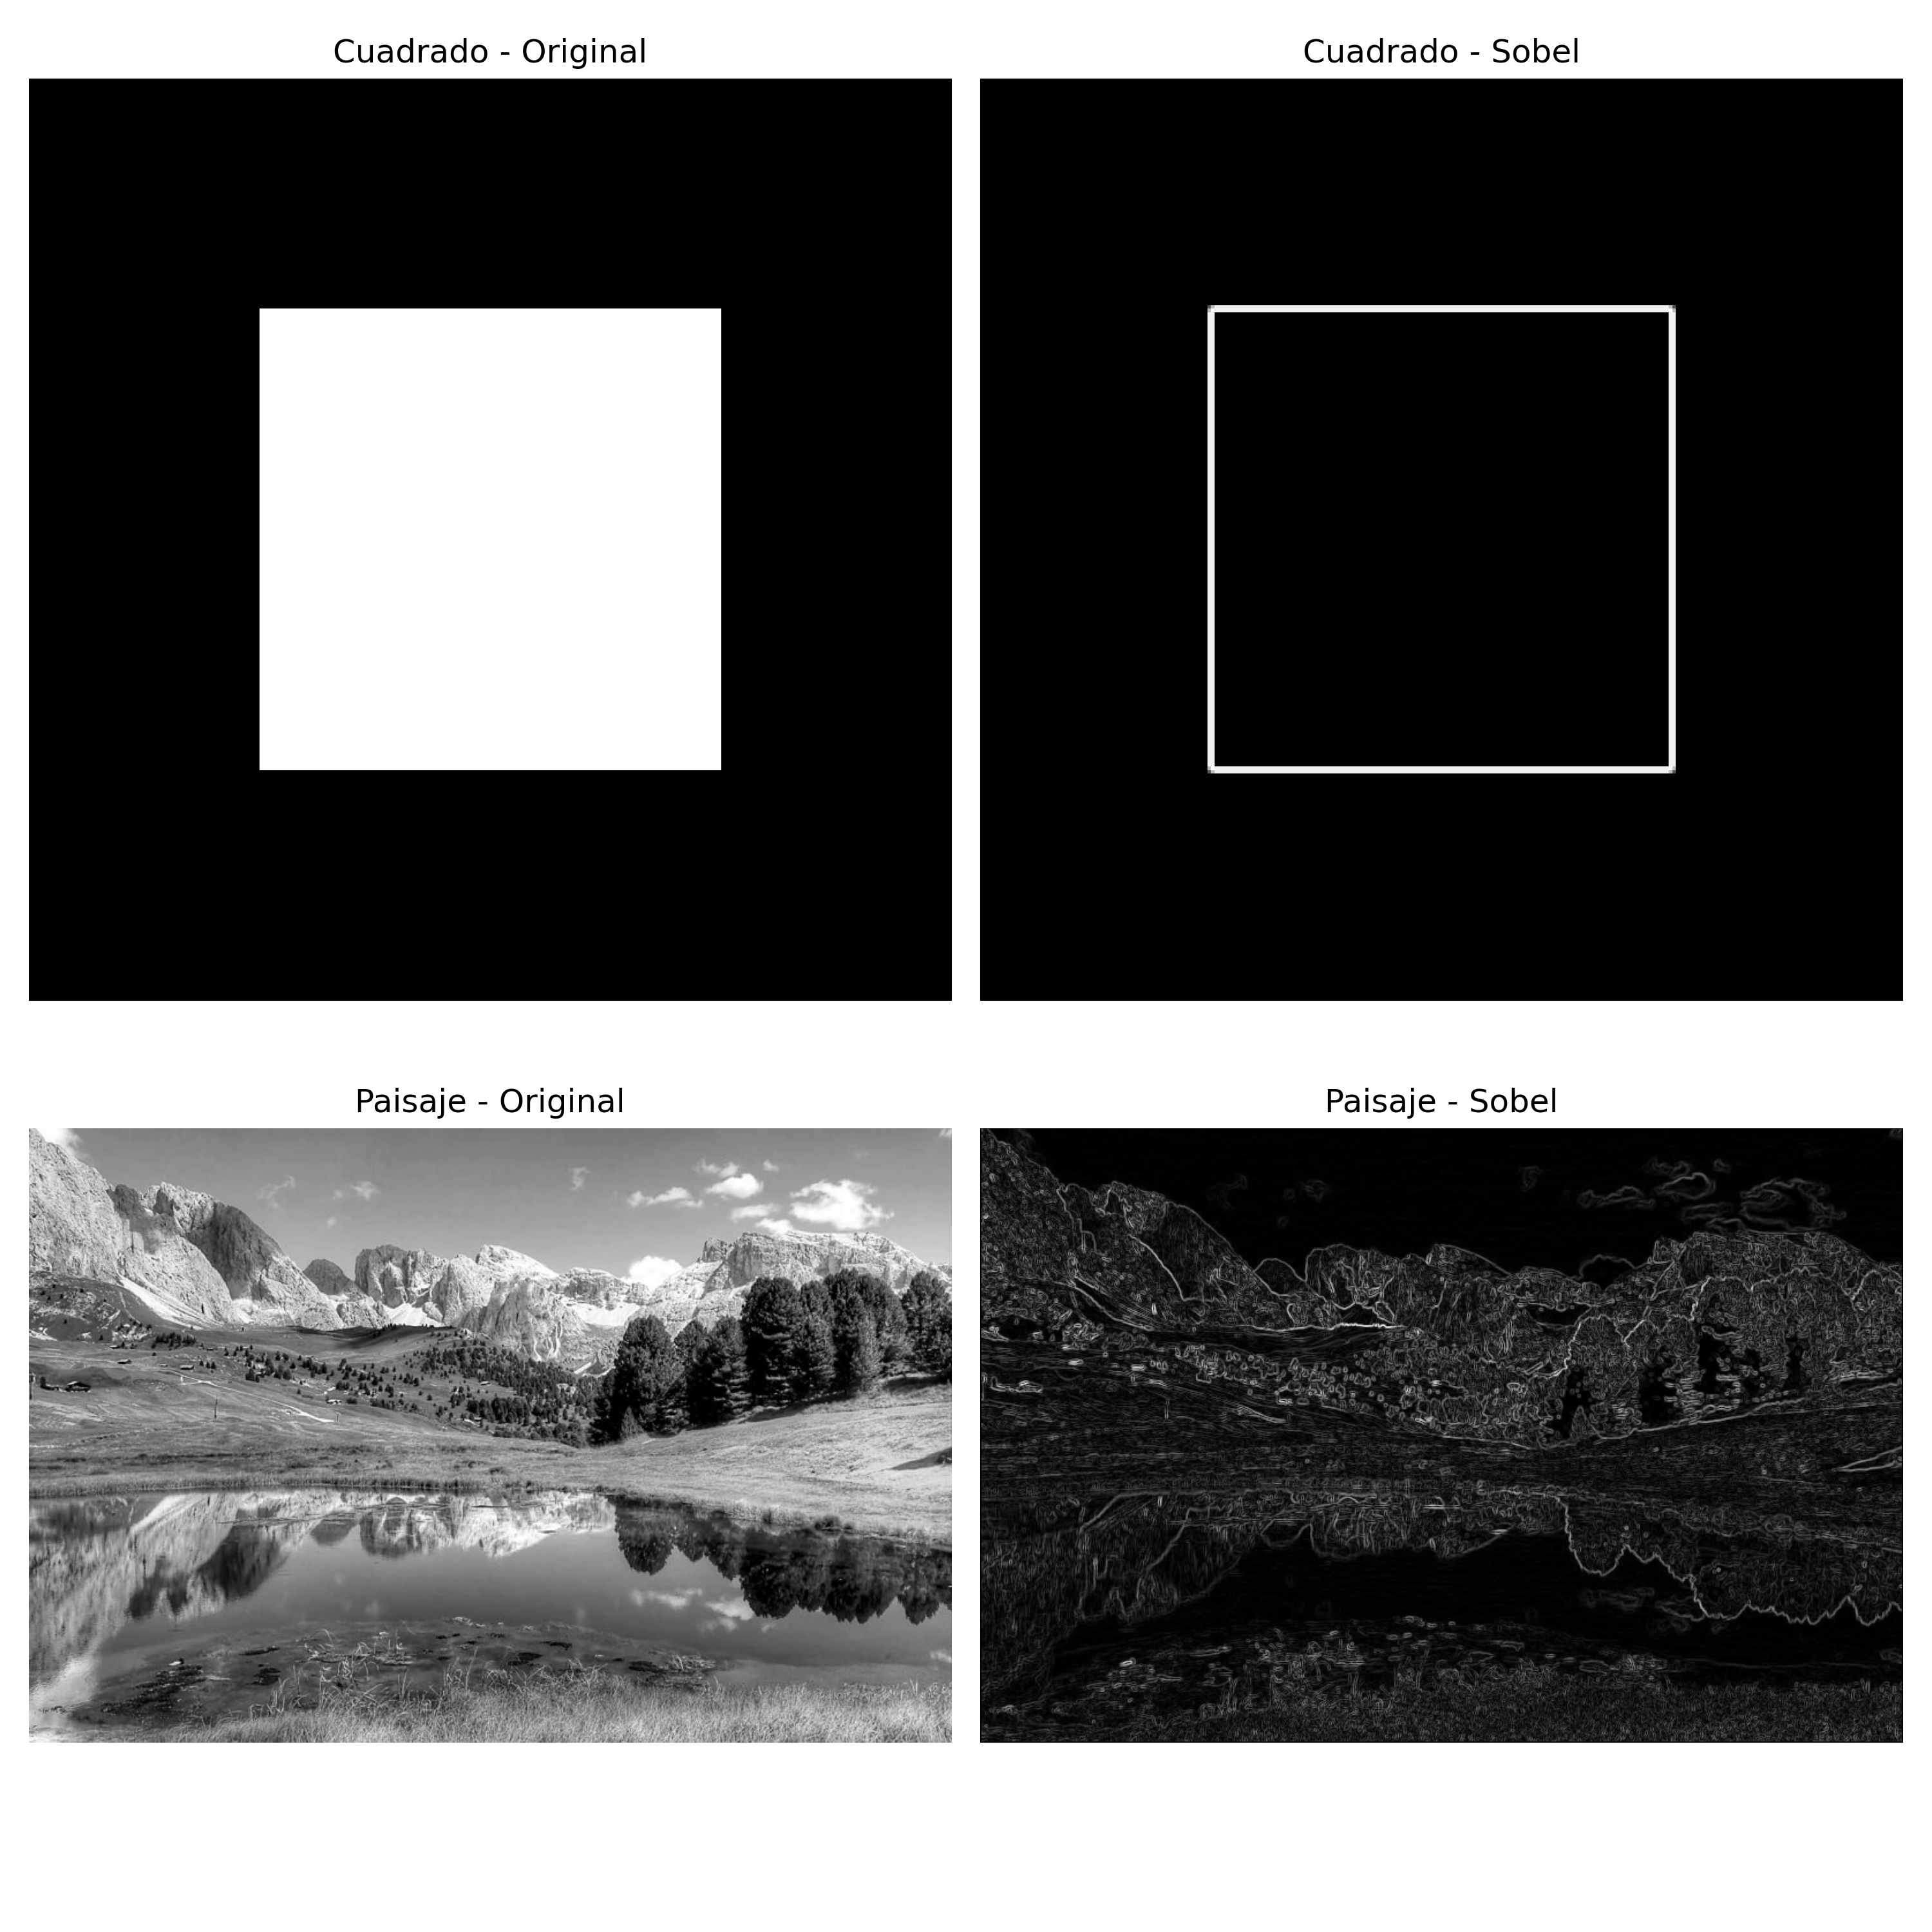
\includegraphics[width=0.90\textwidth]
    {../results/deteccion_bordes_sobel.png}
    \caption{Detección de bordes
    mediante el operador Sobel.}
    \label{fig:sobel}
\end{figure}

En el cuadrado se detectaron
los cuatro contornos, con un
resultado visualmente muy similar
al de Prewitt.

En el paisaje se destacaron
montañas, árboles, vegetación
y reflejos. Algunas respuestas
parecieron ligeramente más intensas,
pero las diferencias visuales
fueron pequeñas.

Sobel puede generar respuestas numéricas
mayores debido a los coeficientes
de peso 2.

Sin embargo, esto no representa
por sí mismo una mejor detección,
ya que la escala de las respuestas
también es diferente.

\textbf{Conclusión del punto:}
Sobel permitió detectar correctamente
los bordes, aunque en estas imágenes
no se observó una diferencia visual
considerable respecto a Prewitt.

% ---------------------------------------------------------
\subsection{Punto 5: Detector Laplaciano}

\subsubsection*{Objetivo}

Implementar mediante ciclos
un detector de bordes basado
en el operador Laplaciano.

\subsubsection*{Fundamento}

El Laplaciano utiliza derivadas
de segundo orden.

La máscara empleada fue:

\[
L=
\begin{bmatrix}
0&1&0\\
1&-4&1\\
0&1&0
\end{bmatrix}
\]

A diferencia de Prewitt y Sobel,
no calcula por separado las dos
componentes del gradiente.

\subsubsection*{Implementación}

\begin{lstlisting}
def detectar_bordes_laplaciano(imagen):

    if imagen is None:
        raise ValueError(
            "La imagen no se cargo"
        )

    filas, columnas = imagen.shape

    mascara = np.array([
        [0,  1, 0],
        [1, -4, 1],
        [0,  1, 0]
    ])

    respuestas = np.zeros(
        (filas, columnas),
        dtype=np.float64
    )

    for fila in range(1, filas - 1):
        for columna in range(1, columnas - 1):

            suma = 0.0

            for i in range(-1, 2):
                for j in range(-1, 2):

                    pixel = float(
                        imagen[fila+i, columna+j]
                    )

                    peso = mascara[i+1, j+1]

                    suma += pixel * peso

            respuestas[fila, columna] = suma

    return respuestas
\end{lstlisting}

\subsubsection*{Resultados y análisis}

\begin{figure}[H]
    \centering
    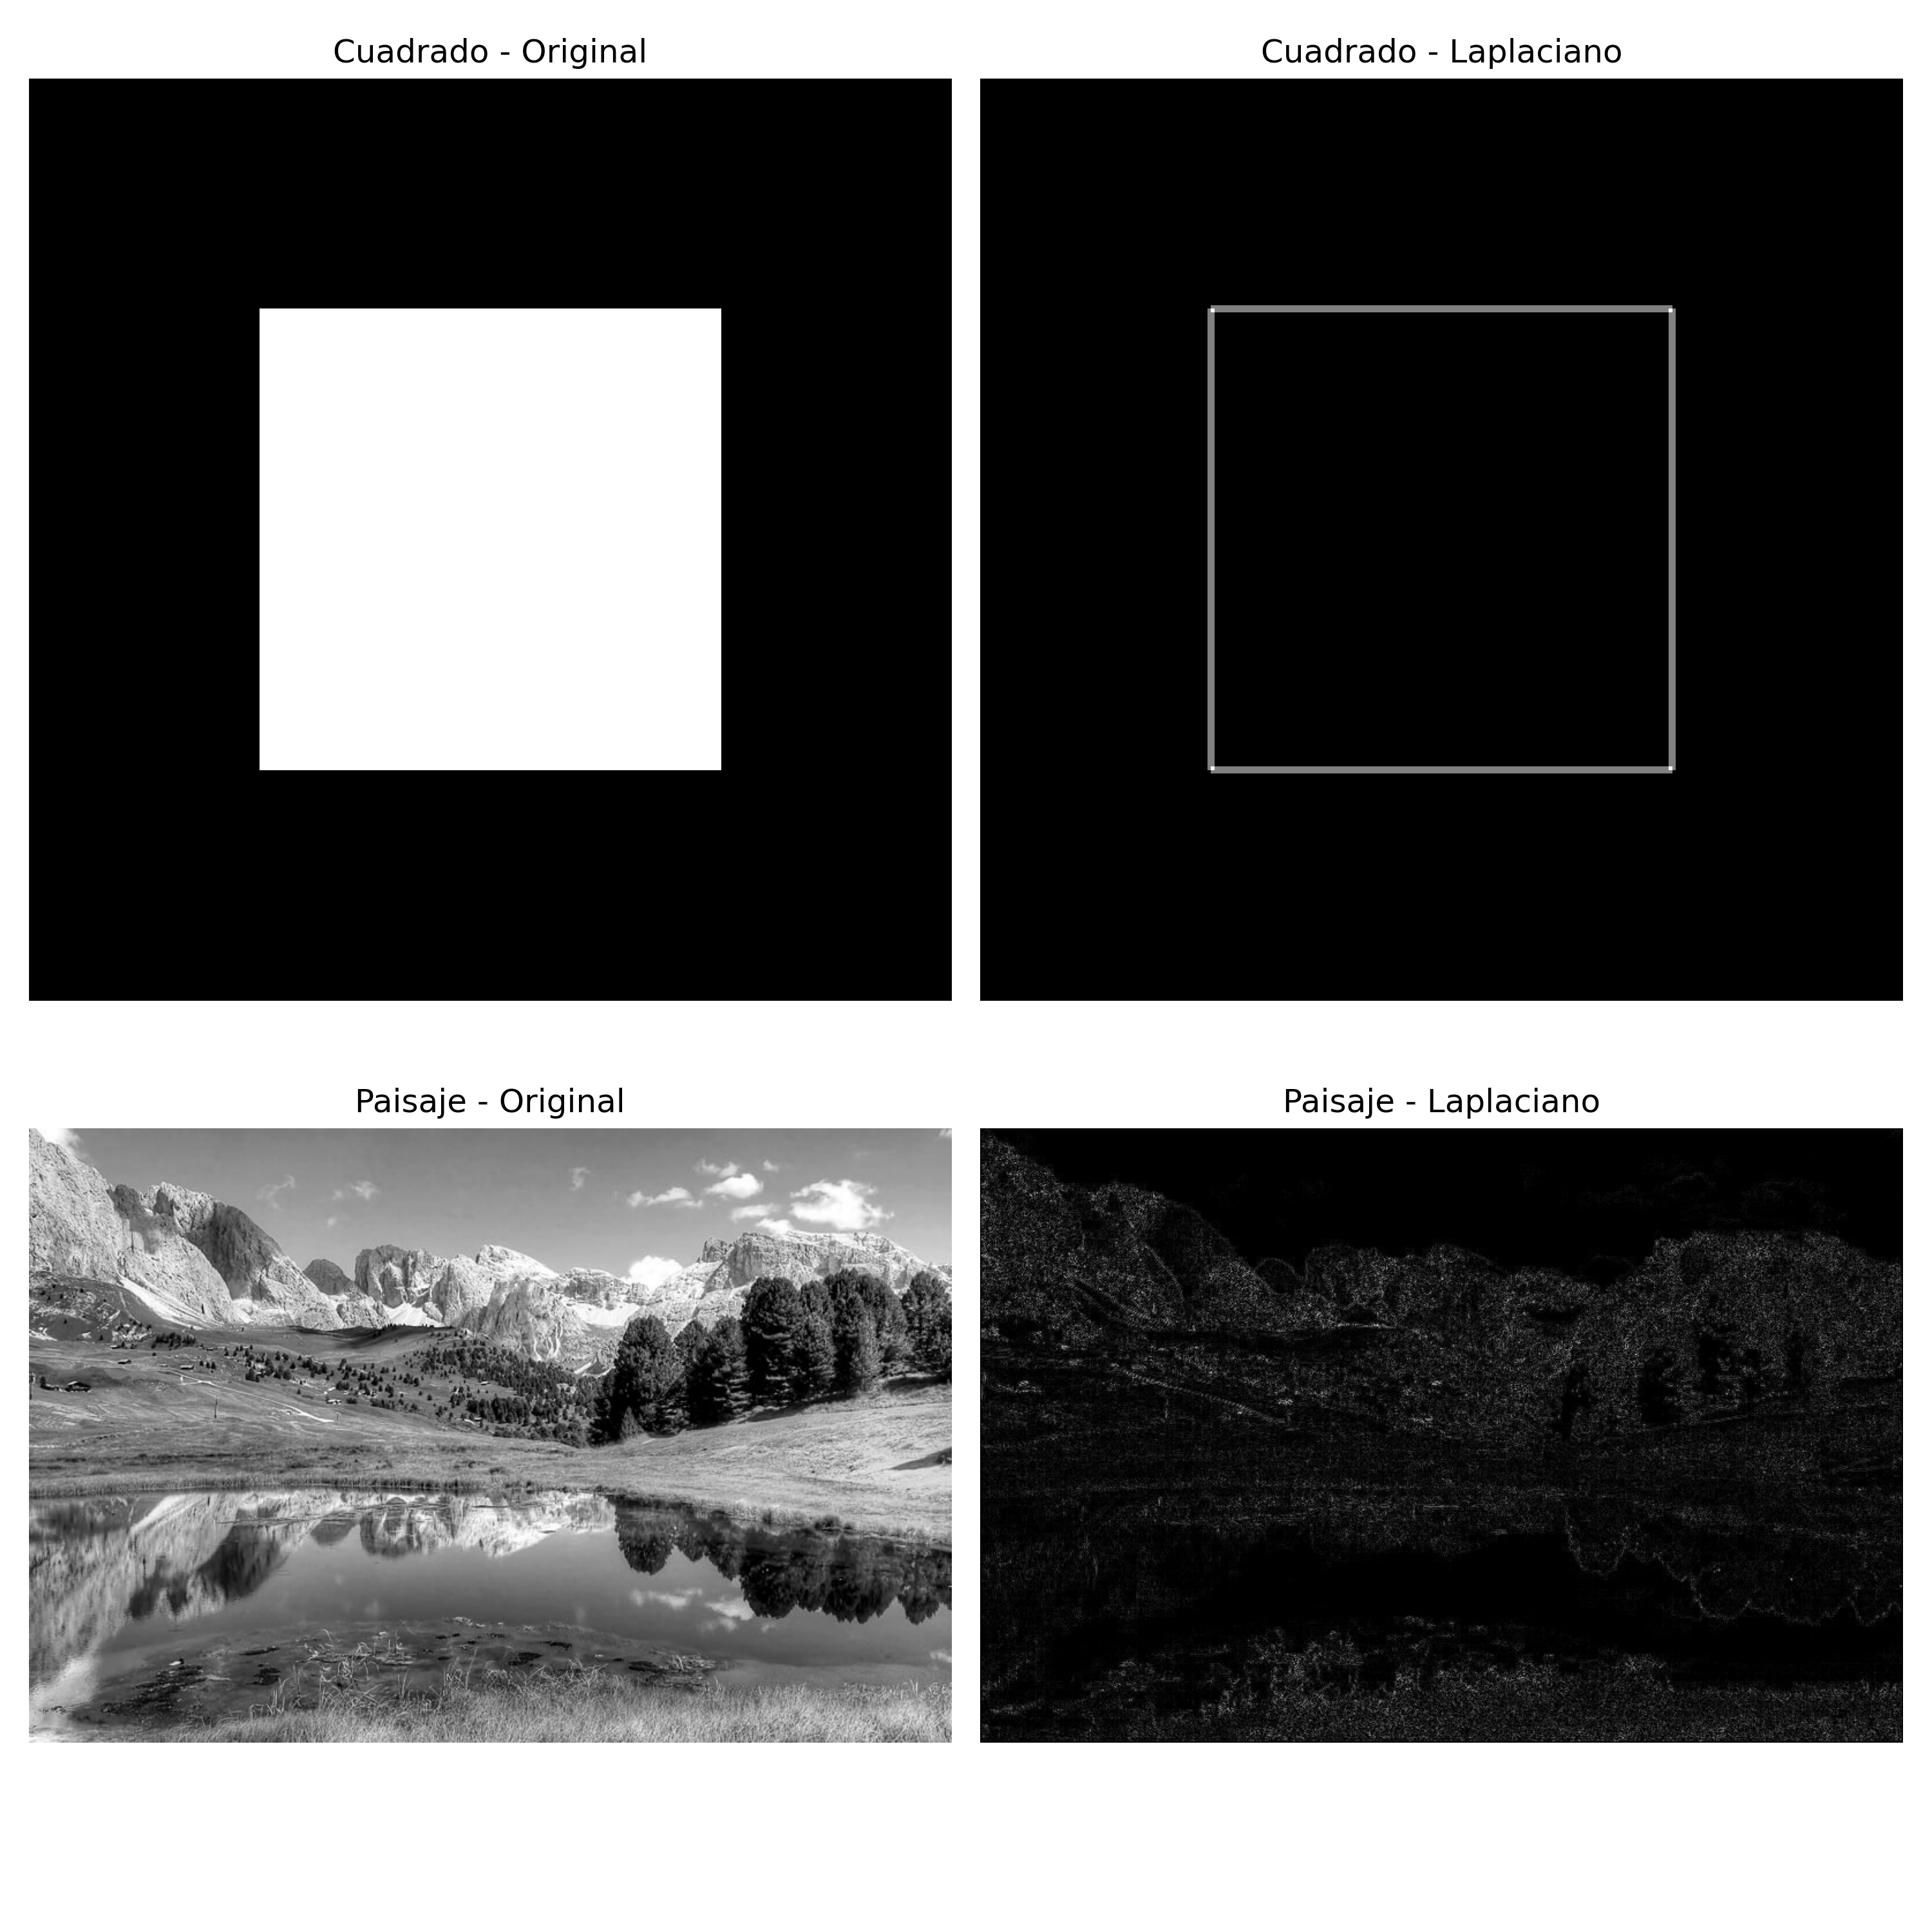
\includegraphics[width=0.90\textwidth]
    {../results/deteccion_bordes_laplaciano.png}
    \caption{Respuestas del Laplaciano
    sobre el cuadrado y el paisaje.}
    \label{fig:laplaciano}
\end{figure}

En el cuadrado se detectaron los
cuatro lados de la figura.

Para visualizar los resultados
se utilizó el valor absoluto de
las respuestas, debido a que el
Laplaciano produce valores
positivos y negativos.

En el paisaje aparecieron numerosas
respuestas pequeñas, asociadas
con texturas y cambios locales.

Algunos contornos principales fueron
menos claros que con los detectores
basados en gradiente.

\textbf{Conclusión del punto:}
el Laplaciano identifica cambios
de intensidad de segundo orden,
pero puede responder intensamente
a pequeñas variaciones y ruido.

Por esta razón resulta útil combinarlo
con un suavizado previo.

% ---------------------------------------------------------
\subsection{Punto 6: Detector Marr-Hildreth}

\subsubsection*{Objetivo}

Implementar una versión del algoritmo
Marr-Hildreth mediante suavizado
Gaussiano, Laplaciano y detección
de cruces por cero.

\subsubsection*{Fundamento}

Marr-Hildreth combina:

\[
\text{Gaussiano}
\rightarrow
\text{Laplaciano}
\rightarrow
\text{Cruces por cero}
\]

Su respuesta de segundo orden puede
expresarse como:

\begin{equation}
L(x,y)=
\nabla^2(G_\sigma*f)(x,y)
\end{equation}

Un cruce por cero ocurre cuando
la respuesta Laplaciana cambia
de signo.

Se utilizó un umbral para evitar
marcar cambios demasiado pequeños.

\subsubsection*{Implementación}

Primero se construyó la máscara
Gaussiana mediante ciclos:

\begin{lstlisting}
def crear_mascara_gaussiana(tamano, sigma):

    if tamano <= 0 or tamano % 2 == 0:
        raise ValueError(
            "El tamano debe ser impar"
        )

    if sigma <= 0:
        raise ValueError(
            "Sigma debe ser positivo"
        )

    mascara = np.zeros(
        (tamano, tamano),
        dtype=np.float64
    )

    radio = tamano // 2

    for i in range(-radio, radio+1):
        for j in range(-radio, radio+1):

            mascara[i+radio, j+radio] = np.exp(
                -(i**2+j**2) / (2*sigma**2)
            )

    mascara = mascara / np.sum(mascara)

    return mascara
\end{lstlisting}

Después se implementó el suavizado:

\begin{lstlisting}
def suavizado_gaussiano(
    imagen, sigma=2, tamano=5
):

    mascara = crear_mascara_gaussiana(
        tamano, sigma
    )

    filas, columnas = imagen.shape
    radio = tamano // 2

    extendida = np.pad(
        imagen.astype(np.float64),
        radio,
        mode="edge"
    )

    resultado = np.zeros(
        (filas, columnas),
        dtype=np.float64
    )

    for fila in range(filas):
        for columna in range(columnas):

            suma = 0.0

            for i in range(tamano):
                for j in range(tamano):

                    pixel = extendida[
                        fila+i, columna+j
                    ]

                    suma += (
                        pixel * mascara[i, j]
                    )

            resultado[fila, columna] = suma

    return resultado
\end{lstlisting}

Se implementó un detector sencillo
de cruces por cero que compara
pares opuestos de vecinos:

\begin{lstlisting}
def detectar_cruces_cero(laplaciano, umbral):

    filas, columnas = laplaciano.shape

    bordes = np.zeros(
        (filas, columnas),
        dtype=np.uint8
    )

    for fila in range(1, filas-1):
        for columna in range(1, columnas-1):

            pares = [
                (
                    laplaciano[fila, columna-1],
                    laplaciano[fila, columna+1]
                ),
                (
                    laplaciano[fila-1, columna],
                    laplaciano[fila+1, columna]
                ),
                (
                    laplaciano[fila-1, columna-1],
                    laplaciano[fila+1, columna+1]
                ),
                (
                    laplaciano[fila-1, columna+1],
                    laplaciano[fila+1, columna-1]
                )
            ]

            for a, b in pares:

                if (
                    a*b < 0
                    and abs(a-b) > umbral
                ):
                    bordes[fila, columna] = 255
                    break

    return bordes
\end{lstlisting}

Finalmente se combinaron las etapas,
reutilizando el operador Laplaciano
del punto anterior:

\begin{lstlisting}
def detectar_bordes_marr_hildreth(
    imagen, sigma=2, tamano=5, umbral=10
):

    suavizada = suavizado_gaussiano(
        imagen,
        sigma=sigma,
        tamano=tamano
    )

    laplaciano = detectar_bordes_laplaciano(
        suavizada
    )

    bordes = detectar_cruces_cero(
        laplaciano,
        umbral
    )

    return suavizada, laplaciano, bordes
\end{lstlisting}

\subsubsection*{Resultados y análisis}

\begin{figure}[H]
    \centering
    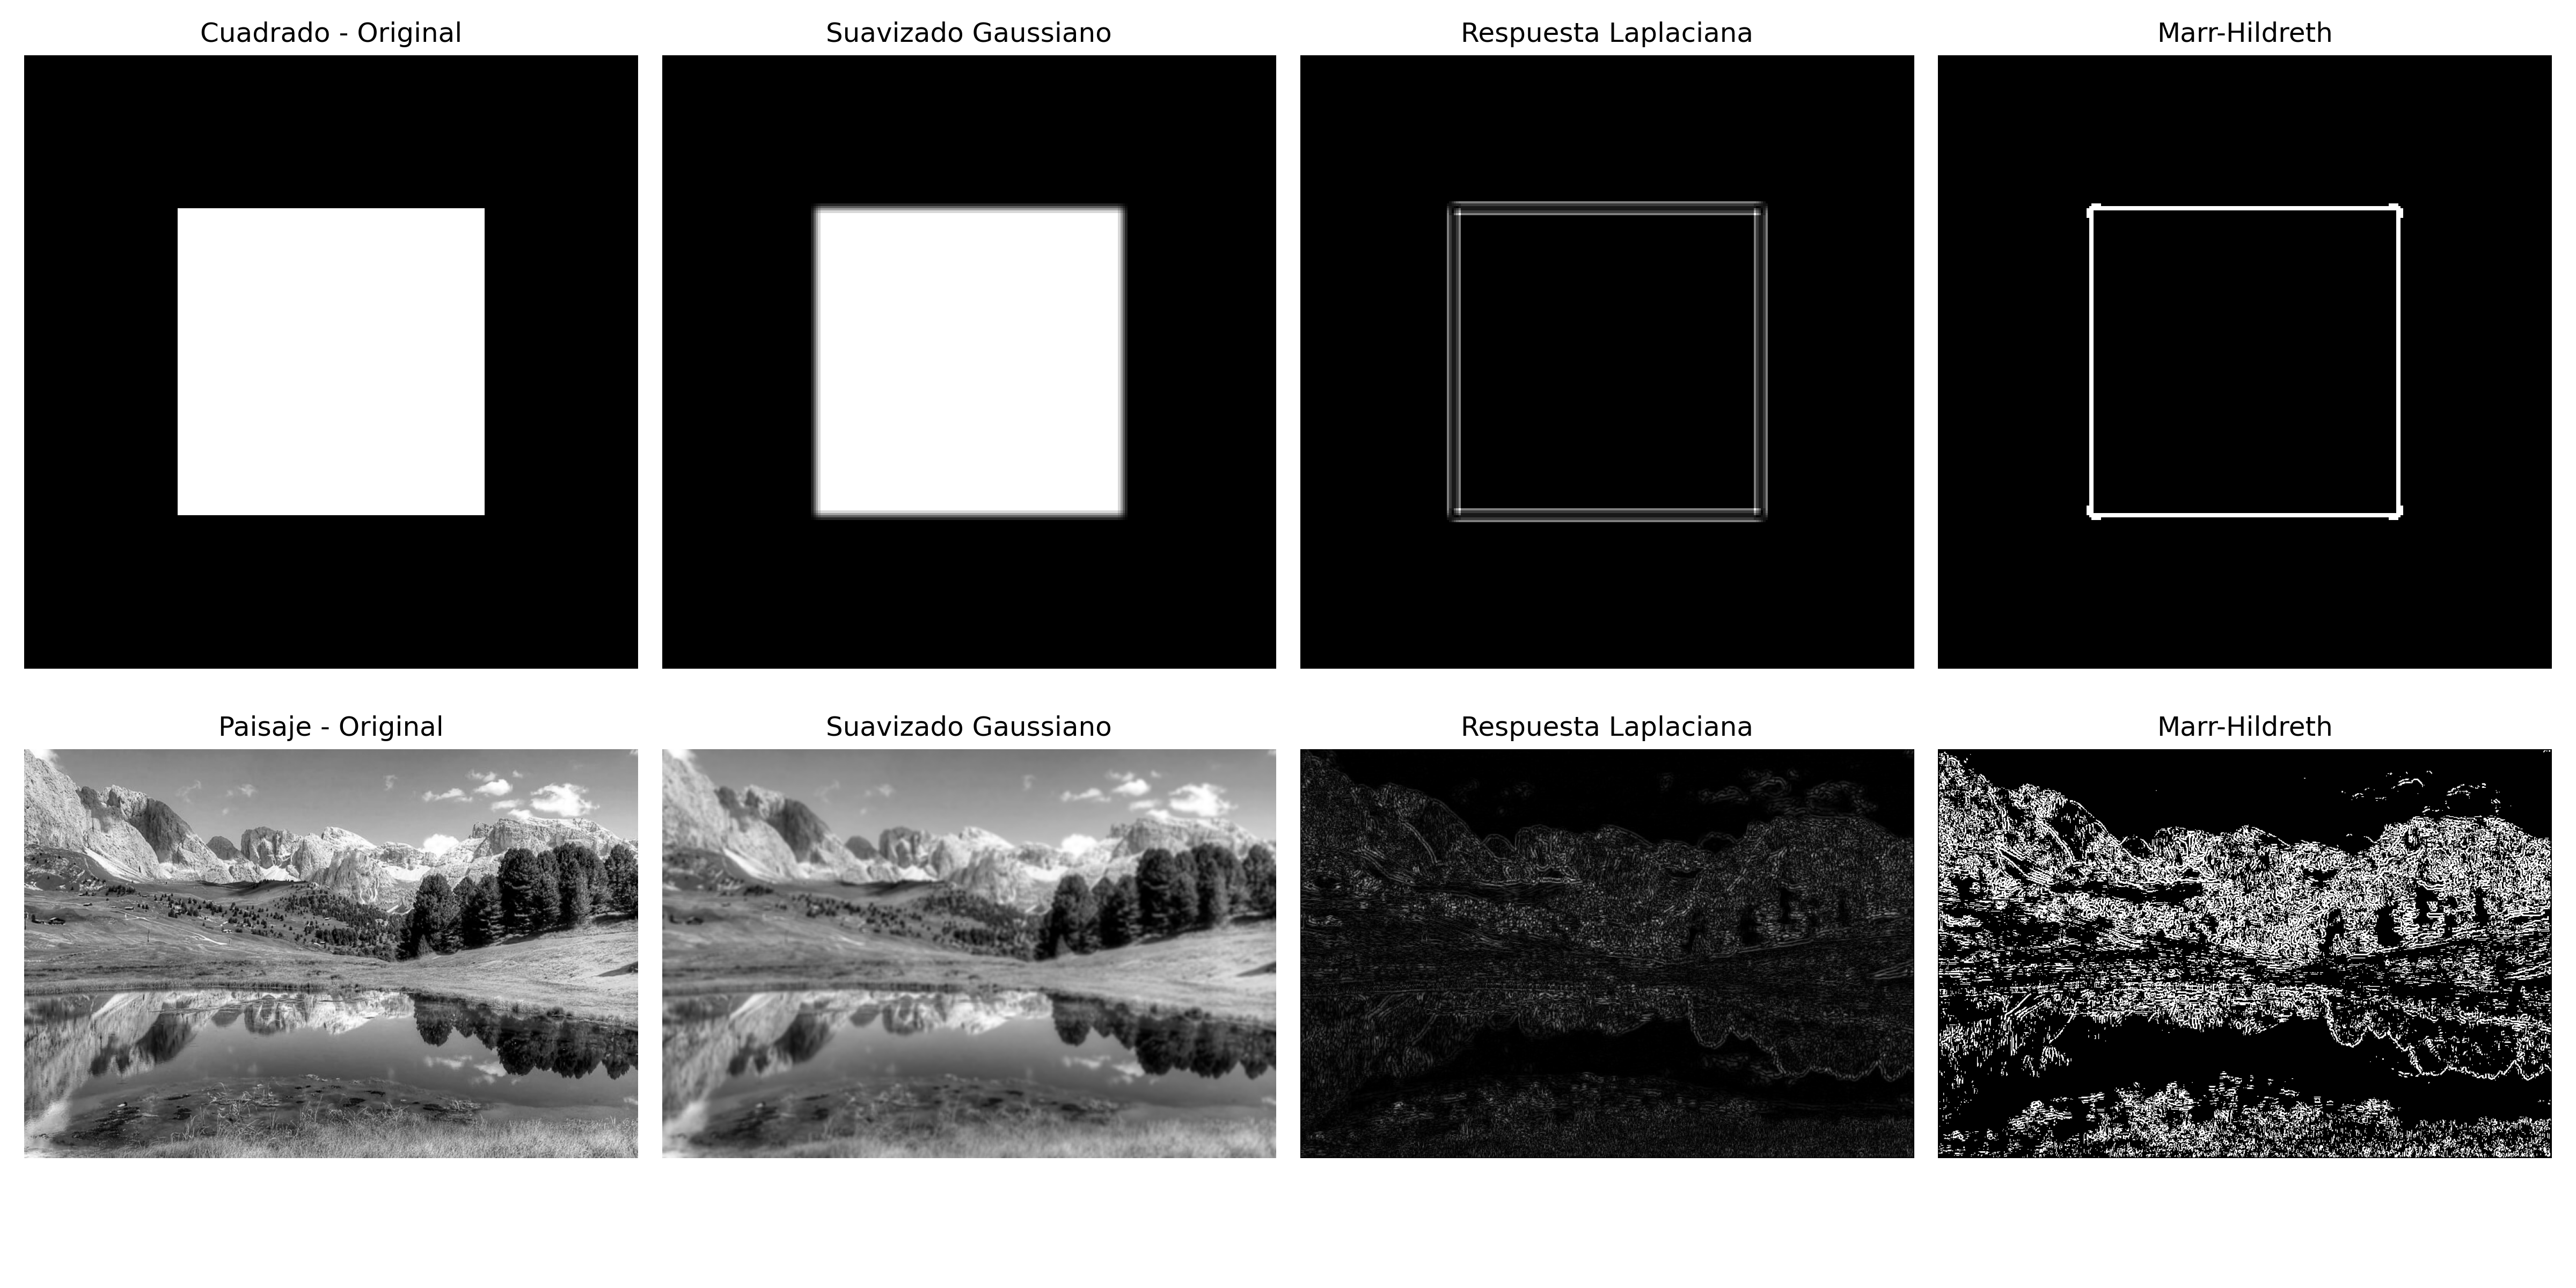
\includegraphics[width=\textwidth]
    {../results/deteccion_bordes_marr_hildreth.png}
    \caption{Etapas del algoritmo Marr-Hildreth
    con $\sigma=2$, máscara de $5\times5$
    y umbral inicial de 10.}
    \label{fig:marr}
\end{figure}

En el cuadrado se obtuvo su contorno
después del suavizado, el Laplaciano
y la detección de cruces por cero.

Algunas esquinas aparecieron ligeramente
más gruesas.

En el paisaje se produjeron numerosas
respuestas, especialmente sobre
montañas, árboles y vegetación.

Para estudiar el efecto del umbral
se probaron valores de 10, 15, 20 y 25.

\begin{figure}[H]
    \centering
    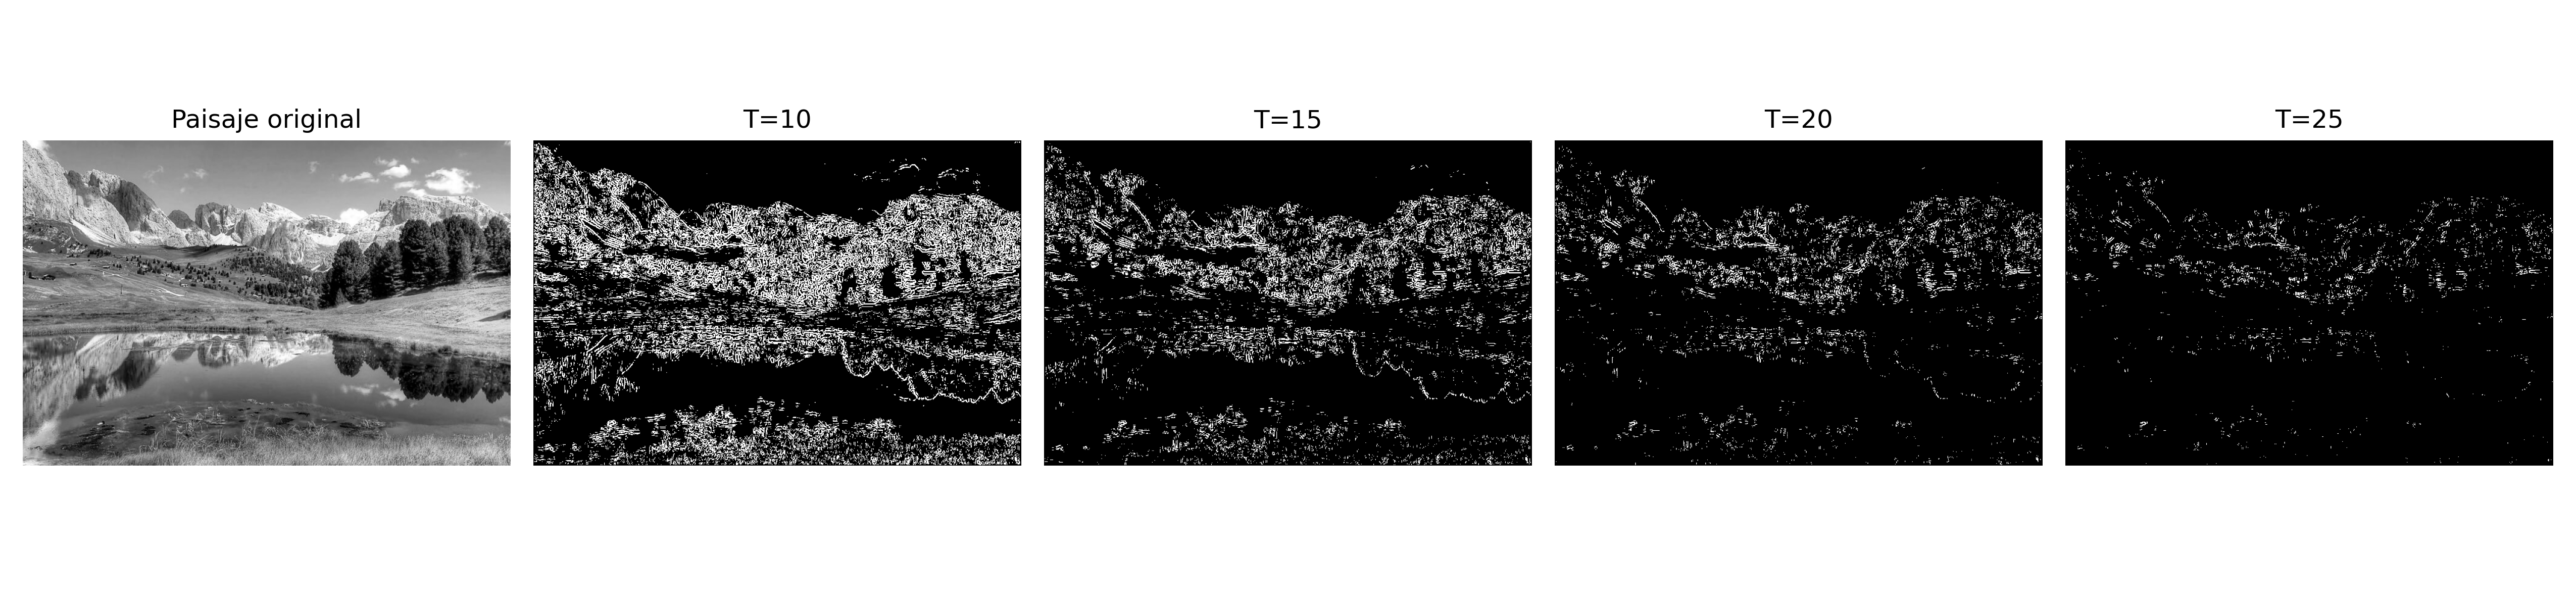
\includegraphics[width=\textwidth]
    {../results/marr_hildreth_umbrales_intermedios.png}
    \caption{Comparación de umbrales
    en Marr-Hildreth aplicado al paisaje.}
    \label{fig:marr_umbrales}
\end{figure}

Con $T=10$ aparecieron demasiadas
detecciones.

Con $T=15$ se conservaron varias
estructuras reconocibles, reduciendo
parte de las respuestas pequeñas.

Con $T=20$ y $T=25$ desaparecieron
más detalles, pero algunos contornos
comenzaron a fragmentarse.

Para este paisaje, $T=15$ ofreció
un equilibrio visual razonable.

\textbf{Conclusión del punto:}
Marr-Hildreth permitió identificar
los límites de una figura geométrica,
pero en imágenes naturales con muchas
texturas produjo numerosas detecciones.

Su resultado depende del suavizado
y del umbral utilizado para identificar
los cruces por cero.

% ---------------------------------------------------------
\subsection{Punto 7: Detector Canny}

\subsubsection*{Objetivo}

Implementar una versión manual del
detector Canny con $\sigma=5$,
utilizando ciclos para las etapas
de procesamiento y selección de bordes.

\subsubsection*{Fundamento}

Canny combina varias operaciones:

\begin{enumerate}

    \item Suavizado Gaussiano.

    \item Cálculo del gradiente
    mediante Sobel.

    \item Supresión de no máximos
    en la dirección del gradiente.

    \item Doble umbral para clasificar
    respuestas fuertes y débiles.

    \item Histéresis para conservar
    bordes débiles conectados
    con bordes fuertes.

\end{enumerate}

La supresión de no máximos reduce
el grosor de las respuestas.

La histéresis ayuda a seleccionar
contornos según su intensidad
y conectividad.

\subsubsection*{Implementación}

Se reutilizaron las funciones
de suavizado Gaussiano y Sobel
desarrolladas anteriormente.

La orientación del gradiente
se calculó mediante:

\begin{lstlisting}
angulo = np.arctan2(gy, gx)
\end{lstlisting}

Se implementó la supresión
de no máximos utilizando cuatro
direcciones aproximadas:

\begin{lstlisting}
def supresion_no_maximos(magnitud, angulo):

    filas, columnas = magnitud.shape

    resultado = np.zeros(
        (filas, columnas),
        dtype=np.float64
    )

    angulo_grados = np.rad2deg(angulo) % 180

    for fila in range(1, filas-1):
        for columna in range(1, columnas-1):

            direccion = angulo_grados[
                fila, columna
            ]

            actual = magnitud[
                fila, columna
            ]

            if (
                direccion < 22.5
                or direccion >= 157.5
            ):
                a = magnitud[fila, columna-1]
                b = magnitud[fila, columna+1]

            elif direccion < 67.5:
                a = magnitud[fila-1, columna+1]
                b = magnitud[fila+1, columna-1]

            elif direccion < 112.5:
                a = magnitud[fila-1, columna]
                b = magnitud[fila+1, columna]

            else:
                a = magnitud[fila-1, columna-1]
                b = magnitud[fila+1, columna+1]

            if actual >= a and actual >= b:
                resultado[fila, columna] = actual

    return resultado
\end{lstlisting}

La etapa de doble umbral e histéresis
se implementó mediante una lista
de posiciones pendientes.

\begin{lstlisting}
def doble_umbral_histeresis(
    magnitud, umbral_bajo, umbral_alto
):

    if (
        umbral_bajo < 0
        or umbral_alto <= umbral_bajo
    ):
        raise ValueError(
            "Umbrales no validos"
        )

    filas, columnas = magnitud.shape

    fuertes = magnitud >= umbral_alto
    debiles = magnitud >= umbral_bajo

    bordes = np.zeros(
        (filas, columnas),
        dtype=np.uint8
    )

    pendientes = []

    for fila in range(filas):
        for columna in range(columnas):

            if fuertes[fila, columna]:
                bordes[fila, columna] = 255
                pendientes.append(
                    (fila, columna)
                )

    while pendientes:

        fila, columna = pendientes.pop()

        for i in range(-1, 2):
            for j in range(-1, 2):

                nueva_fila = fila+i
                nueva_columna = columna+j

                if (
                    0 <= nueva_fila < filas
                    and 0 <= nueva_columna < columnas
                ):
                    if (
                        debiles[
                            nueva_fila, nueva_columna
                        ]
                        and bordes[
                            nueva_fila, nueva_columna
                        ] == 0
                    ):
                        bordes[
                            nueva_fila, nueva_columna
                        ] = 255

                        pendientes.append(
                            (nueva_fila, nueva_columna)
                        )

    return bordes
\end{lstlisting}

La función principal integró
las cuatro etapas:

\begin{lstlisting}
def detectar_bordes_canny(
    imagen,
    sigma=5,
    umbral_bajo=50,
    umbral_alto=120
):

    if imagen is None:
        raise ValueError(
            "La imagen no se cargo"
        )

    suavizada = suavizado_gaussiano(
        imagen,
        sigma=sigma,
        tamano=31
    )

    magnitud, gx, gy = detectar_bordes_sobel(
        suavizada
    )

    angulo = np.arctan2(gy, gx)

    suprimida = supresion_no_maximos(
        magnitud,
        angulo
    )

    bordes = doble_umbral_histeresis(
        suprimida,
        umbral_bajo,
        umbral_alto
    )

    return (
        suavizada,
        magnitud,
        suprimida,
        bordes
    )
\end{lstlisting}

\subsubsection*{Resultados y análisis}

Primero se utilizó el cuadrado
con $\sigma=5$ y umbrales 50 y 120.

\begin{figure}[H]
    \centering
    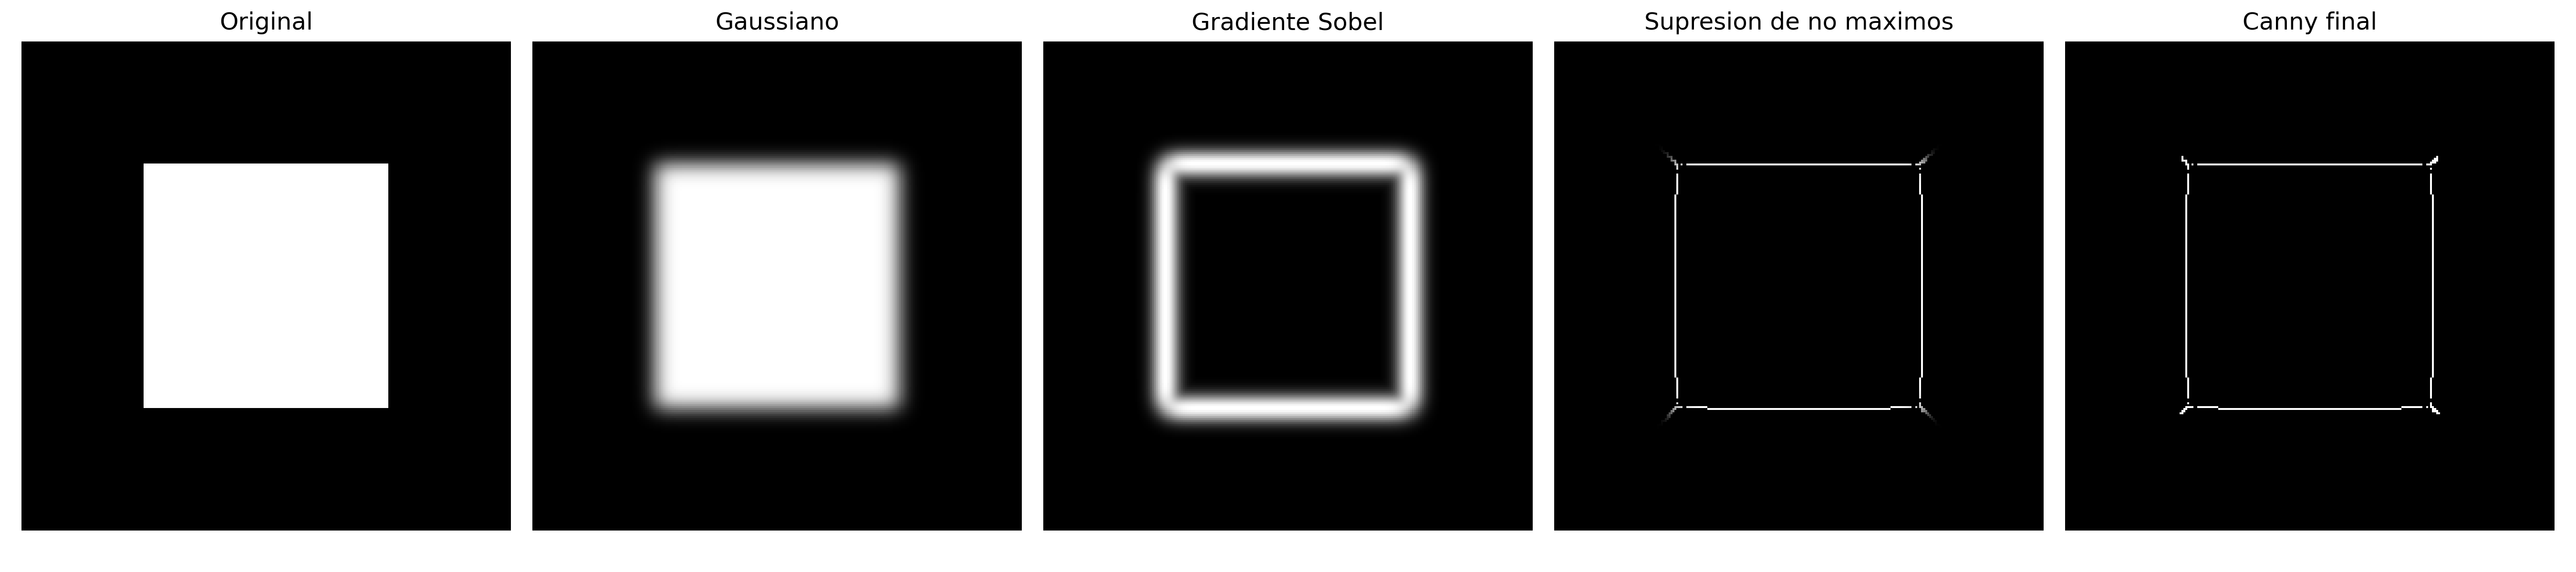
\includegraphics[width=\textwidth]
    {../results/deteccion_bordes_canny_cuadrado.png}
    \caption{Etapas de Canny
    sobre el cuadrado.}
    \label{fig:canny_cuadrado}
\end{figure}

El suavizado hizo menos bruscos
los bordes del cuadrado.

Sobel produjo contornos relativamente
gruesos, mientras que la supresión
de no máximos permitió adelgazarlos.

Finalmente, la histéresis conservó
los cuatro lados de la figura.

Aparecieron pequeñas interrupciones
y ramificaciones en las esquinas,
relacionadas con la aproximación
del gradiente a cuatro direcciones.

Posteriormente se aplicó Canny
al paisaje con $\sigma=5$.

Inicialmente se utilizaron umbrales
50 y 120, pero el resultado
quedó completamente negro.

Al revisar las magnitudes
se obtuvieron los siguientes valores:

\begin{table}[H]
\centering
\caption{Magnitudes obtenidas en el paisaje.}
\begin{tabular}{lc}
\toprule
\textbf{Medición} & \textbf{Resultado}\\
\midrule
Máximo del gradiente Sobel & 109,60\\
Máximo después de supresión & 109,60\\
Píxeles con magnitud $\geq120$ & 0\\
Píxeles con magnitud $\geq50$ & 1816\\
\bottomrule
\end{tabular}
\end{table}

Como ningún píxel superaba
el umbral alto de 120,
la histéresis no encontraba
bordes fuertes para comenzar
el seguimiento.

Por esta razón se probaron
umbrales más bajos.

\begin{figure}[H]
    \centering
    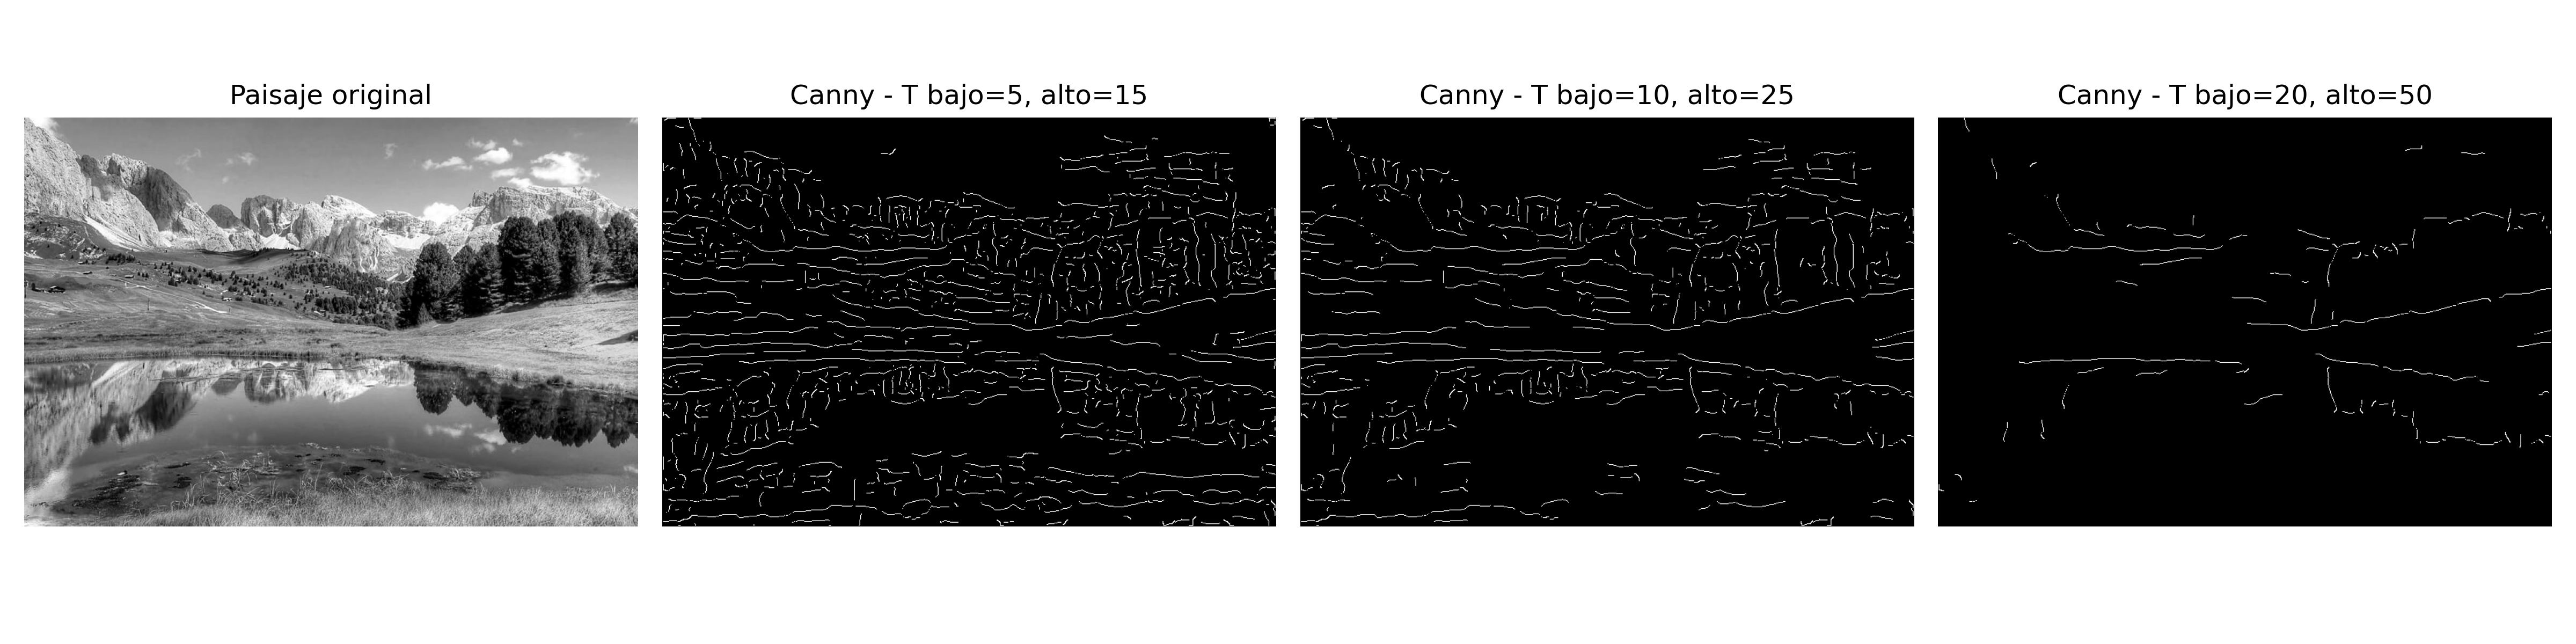
\includegraphics[width=\textwidth]
    {../results/canny_comparacion_umbrales.png}
    \caption{Comparación de umbrales
    5--15, 10--25 y 20--50.}
    \label{fig:canny_umbrales}
\end{figure}

Con los umbrales 5 y 15
se conservaron numerosas
variaciones del paisaje.

Con 10 y 25 se redujeron
parte de las respuestas pequeñas
y se mantuvieron visibles
contornos de montañas,
árboles y reflejos.

Con 20 y 50 el resultado
fue más limpio, pero se
perdieron varios bordes.

Por tanto, se seleccionaron
umbrales 10 y 25 para
la prueba final del paisaje.

\begin{figure}[H]
    \centering
    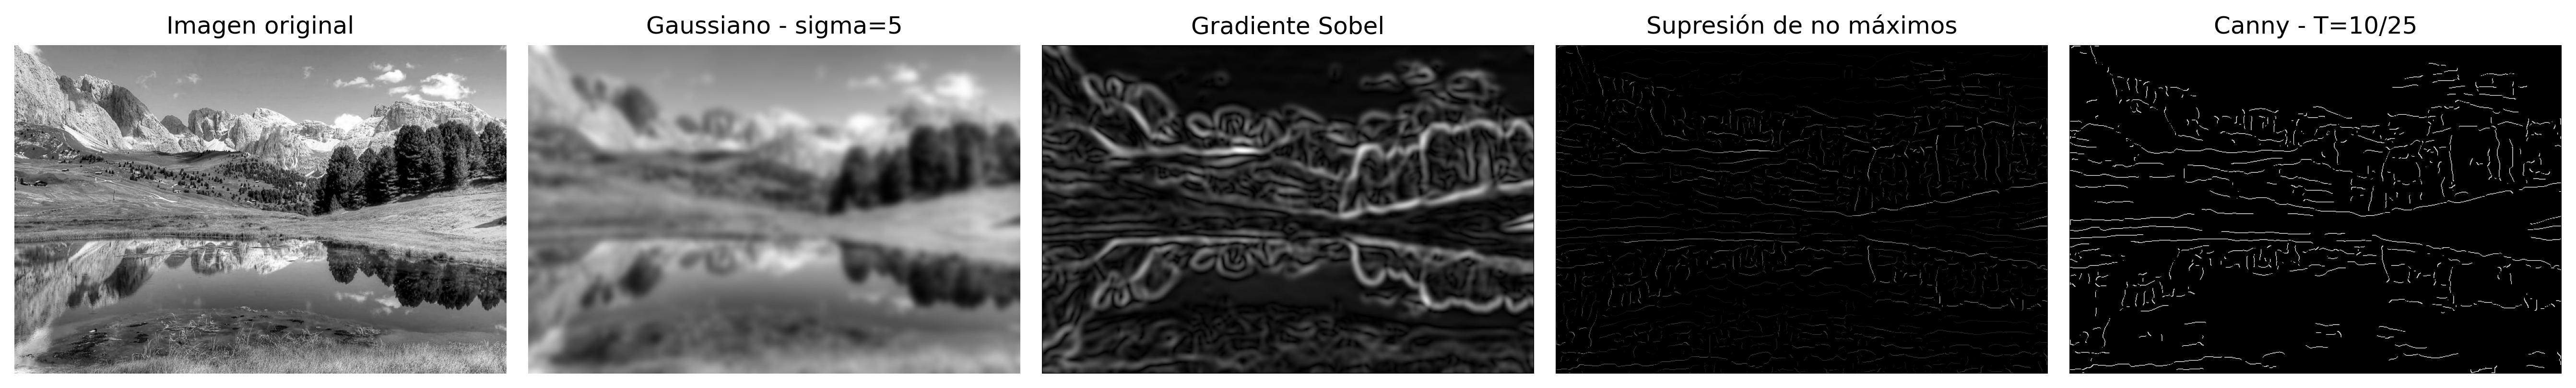
\includegraphics[width=\textwidth]
    {../results/deteccion_bordes_canny_paisaje.png}
    \caption{Etapas de Canny sobre el paisaje
    con $\sigma=5$ y umbrales 10 y 25.}
    \label{fig:canny_paisaje}
\end{figure}

La figura final permite observar
cómo Sobel genera respuestas gruesas
que después son adelgazadas
mediante la supresión de no máximos.

La histéresis conserva
contornos seleccionados del paisaje,
aunque algunas líneas
presentan interrupciones.

\textbf{Conclusión del punto:}
Canny permite combinar suavizado,
gradiente, adelgazamiento y conectividad
para seleccionar bordes.

Los resultados demostraron que los
umbrales deben ajustarse a las
magnitudes obtenidas, ya que valores
demasiado altos pueden eliminar
completamente las detecciones.

% =========================================================
\section{Análisis general}

El desarrollo del taller permitió
comprender diferentes formas de
detectar características en imágenes
mediante cambios de intensidad.

Los primeros ejercicios mostraron
cómo la distribución de los coeficientes
de una máscara permite identificar
puntos aislados y líneas con
orientaciones específicas.

La comparación del factor $1/9$
demostró que la escala de las respuestas
influye en la cantidad de detecciones
cuando se mantiene un umbral fijo.

Posteriormente, Prewitt y Sobel
permitieron detectar contornos
mediante gradientes horizontales
y verticales.

En las imágenes utilizadas,
ambos produjeron resultados
visualmente muy similares.

El Laplaciano permitió detectar
cambios de segundo orden,
pero produjo numerosas respuestas
sobre las texturas del paisaje.

Esto explicó la utilidad de aplicar
un suavizado previo, como se hizo
en Marr-Hildreth.

En este último algoritmo se observó
que la detección de cruces por cero
depende considerablemente del umbral.

Finalmente, Canny permitió obtener
contornos más delgados mediante
supresión de no máximos y seleccionar
respuestas mediante histéresis.

La prueba del paisaje mostró
la importancia de escoger umbrales
que estén dentro de la escala
de magnitudes calculada.

En conjunto, los resultados evidenciaron
que ningún detector distingue
automáticamente todos los bordes
importantes de una escena.

Las detecciones dependen del algoritmo,
los parámetros y las características
de cada imagen.

% =========================================================
\section{Conclusiones}

Se implementaron siete algoritmos
de detección de características
utilizando principalmente máscaras
espaciales y ciclos en Python.

La detección de puntos aislados
permitió comprobar la influencia
del umbral y del factor $1/9$
sobre la magnitud de las respuestas.

Las máscaras orientadas detectaron
correctamente las cuatro líneas
de la imagen sintética.

Prewitt y Sobel permitieron localizar
bordes mediante gradientes,
con resultados visualmente similares
en las imágenes utilizadas.

El Laplaciano identificó contornos,
pero también numerosas variaciones
pequeñas, mostrando su sensibilidad
a las texturas.

Marr-Hildreth combinó suavizado
y cruces por cero, aunque necesitó
ajustar el umbral para controlar
la cantidad de respuestas.

Finalmente, Canny permitió reducir
el grosor de los bordes y seleccionar
contornos mediante doble umbral
e histéresis.

El taller permitió comprender que
la detección de características
no depende únicamente de aplicar
una máscara, sino también de elegir
adecuadamente los parámetros
y analizar la respuesta obtenida.

\end{document}
